% Options for packages loaded elsewhere
\PassOptionsToPackage{unicode}{hyperref}
\PassOptionsToPackage{hyphens}{url}
\documentclass[
  11pt,
]{article}
\usepackage{xcolor}
\newcommand{\cut}{\textcolor{red}{\textbf{\,[C]}}}  % can cut
\newcommand{\new}[1]{\textcolor{blue}{#1}}  % new text
\usepackage[margin=1in]{geometry}
\usepackage{amsmath,amssymb}
\setcounter{secnumdepth}{-\maxdimen} % remove section numbering
\usepackage{iftex}
\ifPDFTeX
  \usepackage[T1]{fontenc}
  \usepackage[utf8]{inputenc}
  \usepackage{textcomp} % provide euro and other symbols
\else % if luatex or xetex
  \usepackage{unicode-math} % this also loads fontspec
  \defaultfontfeatures{Scale=MatchLowercase}
  \defaultfontfeatures[\rmfamily]{Ligatures=TeX,Scale=1}
\fi
\usepackage{lmodern}
\ifPDFTeX\else
  % xetex/luatex font selection
\fi
% Use upquote if available, for straight quotes in verbatim environments
\IfFileExists{upquote.sty}{\usepackage{upquote}}{}
\IfFileExists{microtype.sty}{% use microtype if available
  \usepackage[]{microtype}
  \UseMicrotypeSet[protrusion]{basicmath} % disable protrusion for tt fonts
}{}
\makeatletter
\@ifundefined{KOMAClassName}{% if non-KOMA class
  \IfFileExists{parskip.sty}{%
    \usepackage{parskip}
  }{% else
    \setlength{\parindent}{0pt}
    \setlength{\parskip}{6pt plus 2pt minus 1pt}}
}{% if KOMA class
  \KOMAoptions{parskip=half}}
\makeatother
\usepackage{graphicx}
\makeatletter
\newsavebox\pandoc@box
\newcommand*\pandocbounded[1]{% scales image to fit in text height/width
  \sbox\pandoc@box{#1}%
  \Gscale@div\@tempa{\textheight}{\dimexpr\ht\pandoc@box+\dp\pandoc@box\relax}%
  \Gscale@div\@tempb{\linewidth}{\wd\pandoc@box}%
  \ifdim\@tempb\p@<\@tempa\p@\let\@tempa\@tempb\fi% select the smaller of both
  \ifdim\@tempa\p@<\p@\scalebox{\@tempa}{\usebox\pandoc@box}%
  \else\usebox{\pandoc@box}%
  \fi%
}
% Set default figure placement to htbp
\def\fps@figure{htbp}
\makeatother
\setlength{\emergencystretch}{3em} % prevent overfull lines
\providecommand{\tightlist}{%
  \setlength{\itemsep}{0pt}\setlength{\parskip}{0pt}}
\usepackage{bookmark}
\IfFileExists{xurl.sty}{\usepackage{xurl}}{} % add URL line breaks if available
\urlstyle{same}
% fallback for those not using the hyperref driver hyperxmp:
\makeatletter
\@ifundefined{xmpquote}{\newcommand{\xmpquote}[1]{#1}}{}
\makeatother
\hypersetup{
  pdftitle={Neural correlates of the word-onset response in human iEEG},
  pdfauthor={Juee Naik, Michael J. Kahana},
  hidelinks,
  pdfcreator={LaTeX via pandoc}}

\title{Neural correlates of the word-onset response in human iEEG}
\author{Juee Naik, Michael J. Kahana}
\date{}

\begin{document}
\maketitle

\subsection{Introduction}\label{introduction}

\subsubsection{The word-onset response in free recall}\label{intro-word-onset}

Most intracranial EEG (iEEG) studies of free recall contrast words that
are later recalled with words that are forgotten (the subsequent memory
effect, SME), or study the retrieval period. As both conditions contain a word, this
contrast measures how responses differ with later memory, but cancels
out the response to the word itself. Only a few studies have examined
the word-onset response directly. Kucewicz et
al.~(2019) showed that high gamma (HG) activity after word onset moves from visual cortex to
the medial temporal lobe (MTL) and then to prefrontal cortex, and Marks
et al.~(2021) found that theta, alpha/beta and gamma activity each
spread across regions on their own timelines during word encoding.

\subsubsection{High gamma and alpha as markers of cortical engagement}\label{intro-hg-alpha}

Broadband HG (70--150 Hz) is widely used as a measure of local population
spiking (Manning et al.~2009; Ray \& Maunsell 2011) and is better described
as a broadband signal than as an oscillation (Burke, Ramayya \& Kahana 2015).
At stimulus onset, alpha and beta power decrease (event-related
desynchronization; Pfurtscheller \& Lopes da Silva 1999), which is thought to
release cortex from alpha-mediated inhibition (Jensen \& Mazaheri 2010). An
alpha/beta decrease together with an HG increase is the typical cortical
activation response, first described in sensorimotor cortex (Crone et
al.~1998a, b) and observed in visual cortex (Lachaux et al.~2005), including
for pseudowords and consonant strings (Vidal et al.~2010). 
In successful memory encoding, words later recalled show lower
low-frequency power and higher HFA than words later forgotten (Sederberg et
al.~2003; Long et al.~2014). This broadband tilt also appears outside memory,
during arithmetic (Randazzo et al.~2019, preprint), where it predicts
response speed, mainly in frontal regions (DeHaan et al.~2025, preprint). Not every
region is engaged by a stimulus, however -- alpha increases in task-irrelevant
cortex are thought to actively inhibit it (Jensen \& Mazaheri 2010), and HG
often decreases during tasks in default-mode regions (Ossandón et al.~2011).

\subsubsection{Timing of visual word processing}\label{intro-timing}

Reading a word unfolds in stages: visual features are extracted within about
100 ms (Thorpe et al.~1996), the letter string is recognised as a word at
about 200 ms (Cohen et al.~2000), its sound is activated automatically (Van
Orden 1987), and its meaning is integrated with context at about 400 ms
(Kutas \& Hillyard 1980). These stages map onto a reading network that runs
from occipital cortex through left fusiform gyrus, which contains the visual
word form area (VWFA; Cohen et al.~2000; Dehaene \& Cohen 2011), to temporal,
supramarginal and inferior frontal cortex (Price 2012; Taylor et al.~2013),
with posterior responses to letter strings preceding more anterior responses
to lexical status (Nobre et al.~1994; Allison et al.~1994).

iEEG resolves when each part of this network responds. Gamma activity begins
at about 150 ms in basal temporal cortex, reaches the VWFA at about 200 ms,
and reaches superior temporal and Broca's areas after 400 ms (Mainy et
al.~2008); word-selective ventral temporal electrodes respond at about 150 ms
(Kadipasaoglu et al.~2016); and the effects of word properties move
anteriorly along the ventral stream, with feedback to posterior regions at
250--500 ms (Woolnough et al.~2021). Beyond the ventral stream, MEG shows
responses proceeding from temporal cortex to Broca's area and finally to
orbitofrontal cortex at about 370 ms (Halgren et al.~2002), and MTL neurons
respond later still, at about 270--400 ms (Mormann et al.~2008). Early visual
responses are sharp, whereas later responses are broad, consistent with
feedforward input followed by feedback (Halgren et al.~2006; Ghuman et
al.~2014). However, most intracranial studies of reading record from tens of
patients with sparse, clinically determined coverage, and focus on the
ventral stream, so the order in which regions across the whole brain respond
to a word has not been measured within one large dataset.

\subsubsection{Synchrony between regions}\label{intro-synchrony}

Beyond local power, word onset may change how regions synchronize. Alpha phase synchrony is thought 
to coordinate distant regions (Palva \& Palva 2007), and alpha power can fall while alpha synchrony 
between regions rises (Hanslmayr et al.~2016). In free recall, slow-frequency synchrony increases 
while high-frequency activity desynchronizes during successful encoding and retrieval 
(Burke et al.~2013; Solomon et al.~2017), and theta hubs mark successful retrieval in this dataset 
(Rao et al.~2025). Connectivity measured at stimulus onset is harder to interpret than power: an evoked 
response shared across regions can raise phase and envelope coupling without any interaction between them, 
and subtracting the average evoked response does not fully remove it, because its amplitude and latency 
vary across trials (Truccolo et al.~2002; David et al.~2006). 
We therefore treat synchrony as a secondary analysis.

\subsubsection{Temporal expectation}\label{intro-expectation}

Reaction times and neural responses depend on how long the participant
waits for a stimulus and on the changing probability that it will appear
(the hazard rate; Niemi \& Näätänen 1981; Nobre \& van Ede 2018).
Temporally expected events evoke larger visual responses: in monkey V1,
gamma increases and alpha decreases when a stimulus is expected (Lima et
al.~2011), and expectation speeds and enhances visual processing in
humans (Doherty et al.~2005).
%We found no iEEG study of how a longer inter-stimulus interval (ISI) affects responses during verbal encoding.

\subsubsection{Predicting recall from the word-onset response}\label{intro-recall}

Spectral features recorded while a word is studied predict whether it will be
recalled (L2-regularised logistic regression; Ezzyat et al.~2017, 2018),
although these classifiers partly track general fluctuations in brain state
rather than encoding of the item (Weidemann \& Kahana 2021). Activity before a
stimulus can also predict memory: pre-stimulus hippocampal theta predicts
later recognition but not recall (Merkow et al.~2014), and pre-stimulus MTL
and cortical low-frequency activity predict encoding success in iEEG (Fell et
al.~2011). Comparing recalled with forgotten words region by region, HFA
predicting later recall appears first in visual, fusiform and medial temporal
regions (about 0--500 ms) and later in left inferior frontal, posterior
parietal and ventrolateral temporal cortex (about 400--900 ms; Burke, Long et
al.~2014). These approaches either pool features across the brain and the
whole word period, or test each region and time point for
a difference in mean activity; how well each region's single-trial response predicts recall, 
and when that prediction arises, has not been measured with classifiers.

\subsubsection{The present study}\label{intro-present}

There have been few whole-brain maps of the response to
word onset itself, contrasting each word to a pre-stimulus baseline. With 362
patients, we obtain a complete set of HG onset latencies across all
regions, extending the existing literature. We also test phase (alpha
ciPLV) and envelope (HG AEC-c) coupling in the same data.

\subsection{Methods}\label{methods}

\subsubsection{Data and cohort}\label{data-and-cohort}

\begin{itemize}
\tightlist
\item
  OpenNeuro BIDS releases of the RAM / Penn free-recall data (FR1,
  catFR1) and pyFR, bipolar montage. OpenNeuro ds004789 (FR1), ds004809
  (catFR1), ds004865 (pyFR).
\item
  362 subjects, 1009 sessions: FR1 232 subj / 466 sess, catFR1 212 /
  465, pyFR 38 / 78.
\item
  Bipolar channels whose contacts are \textgreater{} 20 mm apart, and
  flat channels are dropped.
\item
  Exclusions: missing / \textless{} 499 Hz sampling rate, denylist /
  manual, mains-harmonic peak \textgreater{} 5× its neighbours at a
  non-notched frequency (9 sessions, all 100 Hz peaks at 60 Hz sites).
\item
  Contrast: \textbf{word on} (0--600 ms after word onset) vs
  \textbf{word off} (−700 to −100 ms, the blank screen before the same
  word). Words on screen 1600 s; blank between words
  \textasciitilde750-1250 ms.
\end{itemize}

\subsubsection{Preprocessing}\label{preprocessing}

\begin{itemize}
\tightlist
\item
  Word-off and word-on clips loaded separately per word, each with 500
  ms of real data buffer on both sides.
\item
  Resampled to 500 Hz, notch 60 Hz + 120 Hz harmonic (4th-order
  Butterworth, ±2 Hz); buffer cropped before every estimate. (Widmann et
  al.~2015; de Cheveigné \& Nelken 2019; Gramfort et al.~2013; Virtanen
  et al.~2020)
\item
  Why 500 ms buffer: resampling (FFT) and notching each short clip ring
  at its edges for \textgreater{} 50 ms; the ringing is simultaneous
  across channels and biased the amplitude-correlation measure (AEC-c).
  No effect on multitaper alpha (Supplement)
\end{itemize}

\subsubsection{Electrode localization}\label{electrode-localization}

\begin{itemize}
\tightlist
\item
  Bipolar pairs labelled by lab localization default (depth: volumetric;
  grid/strip: surface). (Desikan et al.~2006; Fischl et al.~2002, 2004;
  Avants et al.~2008; Wang et al.~2013; Yushkevich et al.~2015; Azarion
  et al.~2014 (check); bipolar: Mercier et al.~2022; Li et al.~2018)
\item
  12 Burke ROIs: frontal, temporal, parietal, occipital, limbic,
  hippocampus × hemisphere; sub regions = anatomical labels within them.
  (Burke et al.~2013)
\end{itemize}

\subsubsection{Power}\label{power}

\begin{itemize}
\tightlist
\item
  Alpha (8--13 Hz) and 5--100 Hz spectrum: multitaper, 2 Hz bandwidth,
  600 ms windows; spectrum in 10 log-spaced bins (48--52 / 58--62 Hz
  excluded). (Thomson 1982; Slepian 1978; Percival \& Walden 1993;
  Prerau et al.~2017)
\item
  High gamma (70--150 Hz): Hilbert in 8 × 10 Hz sub-bands, each divided
  by its word-off mean, averaged (broadband, every frequency weighted
  equally). (Edwards et al.~2009 (check); Bruns 2004; Manning et
  al.~2009; Ray \& Maunsell 2011)
\item
  Per electrode: Cohen's d of per-trial power, word on vs word off.
  (Cohen 1988; Lakens 2013)
\end{itemize}

\subsubsection{High-gamma latency}\label{high-gamma-latency}

\begin{itemize}
\tightlist
\item
  Responsive electrodes: per-trial high-gamma power word on
  \textgreater{} word off (one-tailed Welch t test, BH-FDR within
  session): 5004 of 122,339 electrode-sessions, 293 subjects. (Welch
  1947; Benjamini \& Hochberg 1995; selection-then-measure: Kriegeskorte
  et al.~2009)
\item
  Latency: trial-mean envelope minus word-off mean, 30 ms smoothing,
  first time it reaches half its peak within 0--800 ms (half-maximum).
  (Kiesel et al.~2008; Liesefeld 2018; filter smearing: VanRullen 2011)
\item
  Subject median per region → mean ± SEM across subjects; 12 ROIs and
  subregions (hemispheres pooled).
\end{itemize}

\subsubsection{Synchrony}\label{synchrony}

\begin{itemize}
\tightlist
\item
  Alpha: ciPLV (MNE \texttt{spectral\_connectivity\_epochs}, multitaper,
  2 Hz bandwidth). (Bruña et al.~2018; Nolte et al.~2004;
  MNE-Connectivity (Zenodo))
\item
  High gamma: AEC-c (70--110 Hz band-pass + Hilbert,
  \texttt{envelope\_correlation}, pairwise orthogonalized, signed, mean
  over trials); 70--110 Hz so the envelope stays below the band
  (Bedrosian). (Hipp et al.~2012; Bedrosian 1963)
\item
  Pairs sharing a contact excluded. (Mercier et al.~2017) Per electrode:
  mean on − off change over all partners (Rao et al.~2025).
\end{itemize}

\subsubsection{Time-resolved network
(epochs)}\label{time-resolved-network-epochs}

\begin{itemize}
\tightlist
\item
  9 overlapping 200 ms epochs every 100 ms, 0--1000 ms (stops before the
  word's offset response at 1600 ms), each minus the mean of three 200
  ms word-off epochs.
\item
  Region pairs with $\geq$ 100 subjects. Hub (Rao): a region's mean change
  over its connections; t across subjects; two-stage FDR
  (Benjamini--Krieger--Yekutieli) over region × epoch. (Benjamini et
  al.~2006; Rubinov \& Sporns 2010)
\item
  Edges: each significant hub's 5 strongest connections (\textbar mean
  change\textbar), either sign; width $\propto$ \textbar t\textbar{} (Solomon et
  al.~2017 style).
\end{itemize}

\subsubsection{\texorpdfstring{Mixed-effects models (R lme4 / emmeans;
\texttt{mixed\_models.R})}{Mixed-effects models (R lme4 / emmeans; mixed\_models.R)}}\label{mixed-effects-models-r-lme4-emmeans-mixed_models.r}

\begin{itemize}
\tightlist
\item
  Latency: latency\_ms \textasciitilde{} lobe + (1\textbar sub) +
  (1\textbar sub:lobe) + (1\textbar sub:region), one row per responsive
  electrode; all 15 lobe pairs, Holm.
\item
  Power: cohens\_d \textasciitilde{} lobe × band + (1 +
  band\textbar sub) + (1\textbar sub:lobe) + (1\textbar sub:lobe:band) +
  (1\textbar sub:region) + (1\textbar sub:label); lobe × band
  interaction contrast per lobe pair, Holm.
\end{itemize}

\subsubsection{Anticipation}\label{anticipation}

\begin{itemize}
\tightlist
\item
  Responsive electrodes (as latency); trials split at the session's
  median blank length; peak (0--800 ms) of the trial-mean high-gamma
  response after long minus short waits; subject mean per ROI,
  one-sample t, BH-FDR over ROIs.
\end{itemize}

\subsubsection{Recall prediction (encoding contrast: recalled vs not
recalled)}\label{recall-prediction-encoding-contrast-recalled-vs-not-recalled}

\begin{itemize}
\tightlist
\item
  High-gamma response (as latency) in 100 ms windows, 0--1000 ms,
  z-scored within session; per subject × lobe ($\geq$ 5 electrodes) × window:
  L2 logistic regression (C = 7.2e-4, Ezzyat et al.~2017), balanced
  class weights, leave-one-session-out (single-session subjects:
  leave-one-list-out); AUC of pooled held-out predictions.
\item
  Across subjects: one-sided t of AUC \textgreater{} 0.5, BH-FDR over
  lobe × window; permutation chance (\textasciitilde0.49) reported only.
\end{itemize}

\subsubsection{Reliability}\label{reliability}

\begin{itemize}
\tightlist
\item
  Subjects' sessions split at random into two halves ($\geq$ 2 sessions per
  half; riley-thesis rules); per half, d (power) or node strength
  (synchrony) averaged per anatomical region; test-retest = Pearson r
  across the subject's regions between halves.
\end{itemize}

\subsubsection{Statistics}\label{statistics}

\begin{itemize}
\tightlist
\item
  Sessions averaged per electrode, electrodes per subject × region ($\geq$ 1
  electrode); one-sample t vs 0 across subjects; BH-FDR within each
  figure / band; $\geq$ 30 subjects per region. (Holmes \& Friston 1998;
  Benjamini \& Hochberg 1995; Seabold \& Perktold 2010)
\end{itemize}

\subsubsection{Validation (simulations, real montages and events, signal
replaced)}\label{validation-simulations-real-montages-and-events-signal-replaced}

\begin{itemize}
\tightlist
\item
  Power: planted high-gamma gain recovered ($\approx$ identity without noise), 0
  elsewhere.
\item
  ciPLV: lagged alpha coupling recovered monotonically; 0 for null,
  zero-lag leak, envelope plant; planted 400--800 ms coupling found only
  at 400--800 ms.
\item
  AEC-c: planted shared envelope recovered (0.16 → 0.39 → 0.59 with
  depth); non-target pairs 0; zero-lag leak rejected; timing correct.
\item
  Spectrum: 60 Hz notch ringing at clip edges (resolved with the 500 ms
  buffer; 64 Hz bin now unbiased).
\end{itemize}

\subsection{Results}\label{results}

\subsubsection{1. Power changes at word
onset}\label{power-changes-at-word-onset}

\begin{figure}
\centering
\pandocbounded{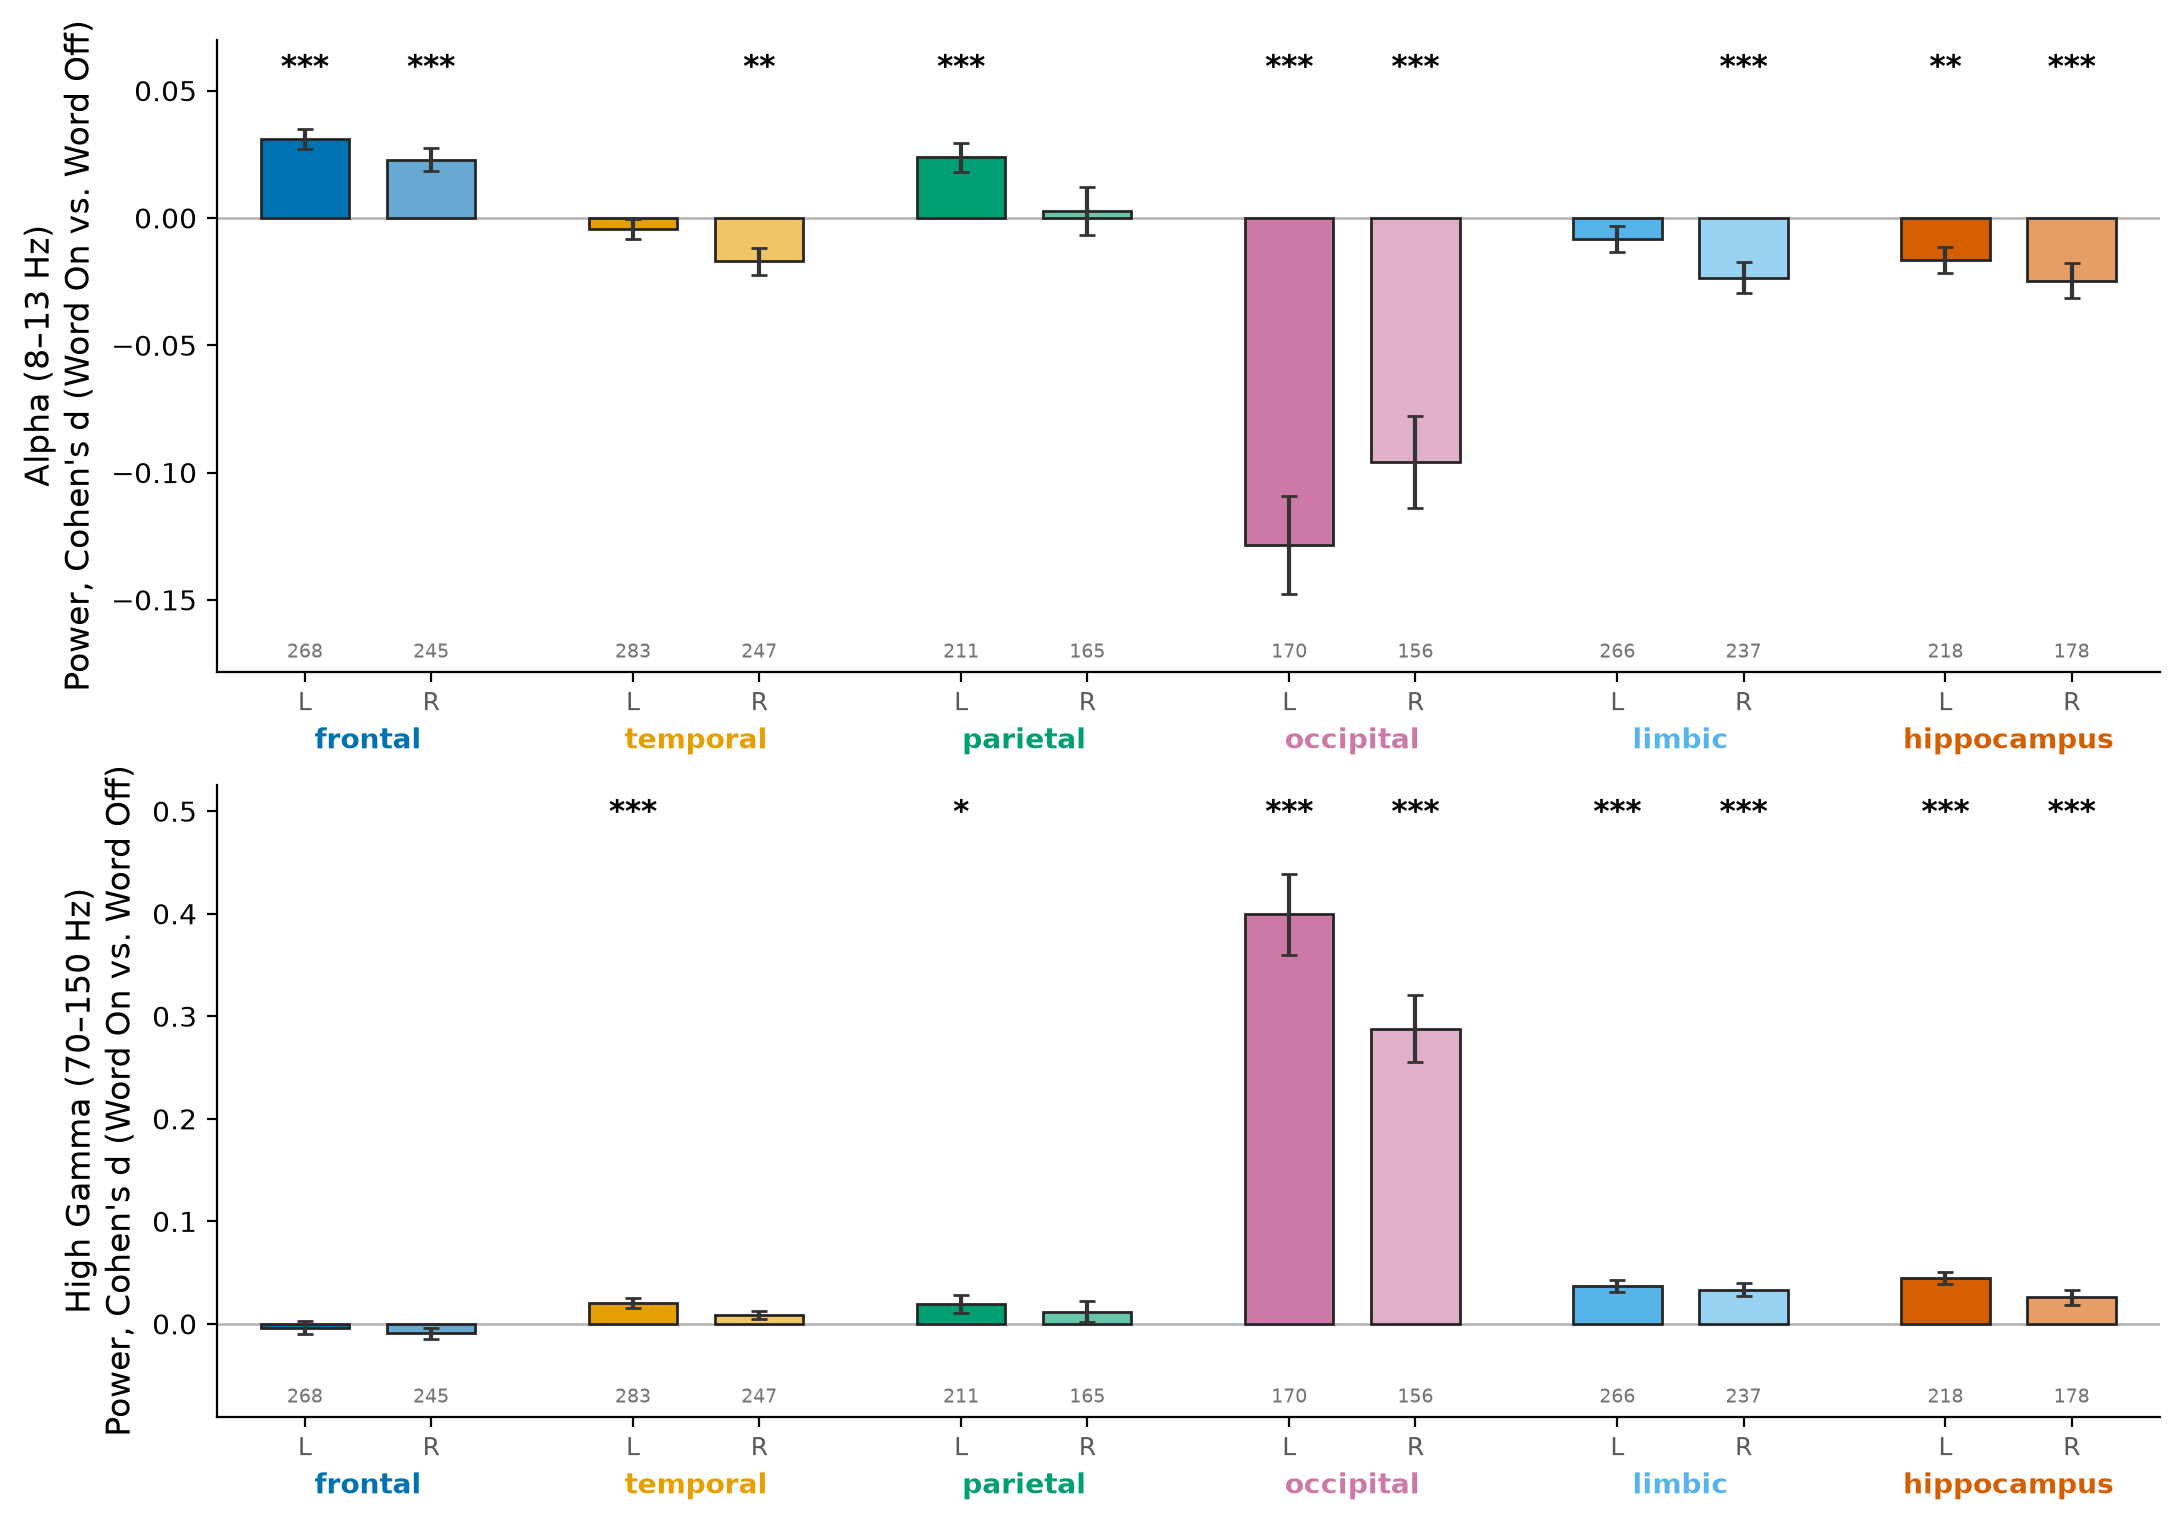
\includegraphics[keepaspectratio,alt={Power per
ROI}]{img/fig1_power.png}}
\caption{Power per ROI}
\end{figure}

\begin{itemize}
\tightlist
\item
  Alpha: decrease in occipital (L −0.14, R −0.11 d), smaller decreases
  in limbic, hippocampus, R temporal; increase in frontal (L +0.031, R
  +0.024) and L parietal (+0.020).
\item
  High gamma: large increase in occipital (L +0.41, R +0.33 d); smaller
  increases in limbic (+0.04), hippocampus (+0.04), L temporal (+0.02);
  slight decrease R frontal (−0.011).
\end{itemize}

\paragraph{Spectral profile}\label{spectral-profile}

\begin{figure}
\centering
\pandocbounded{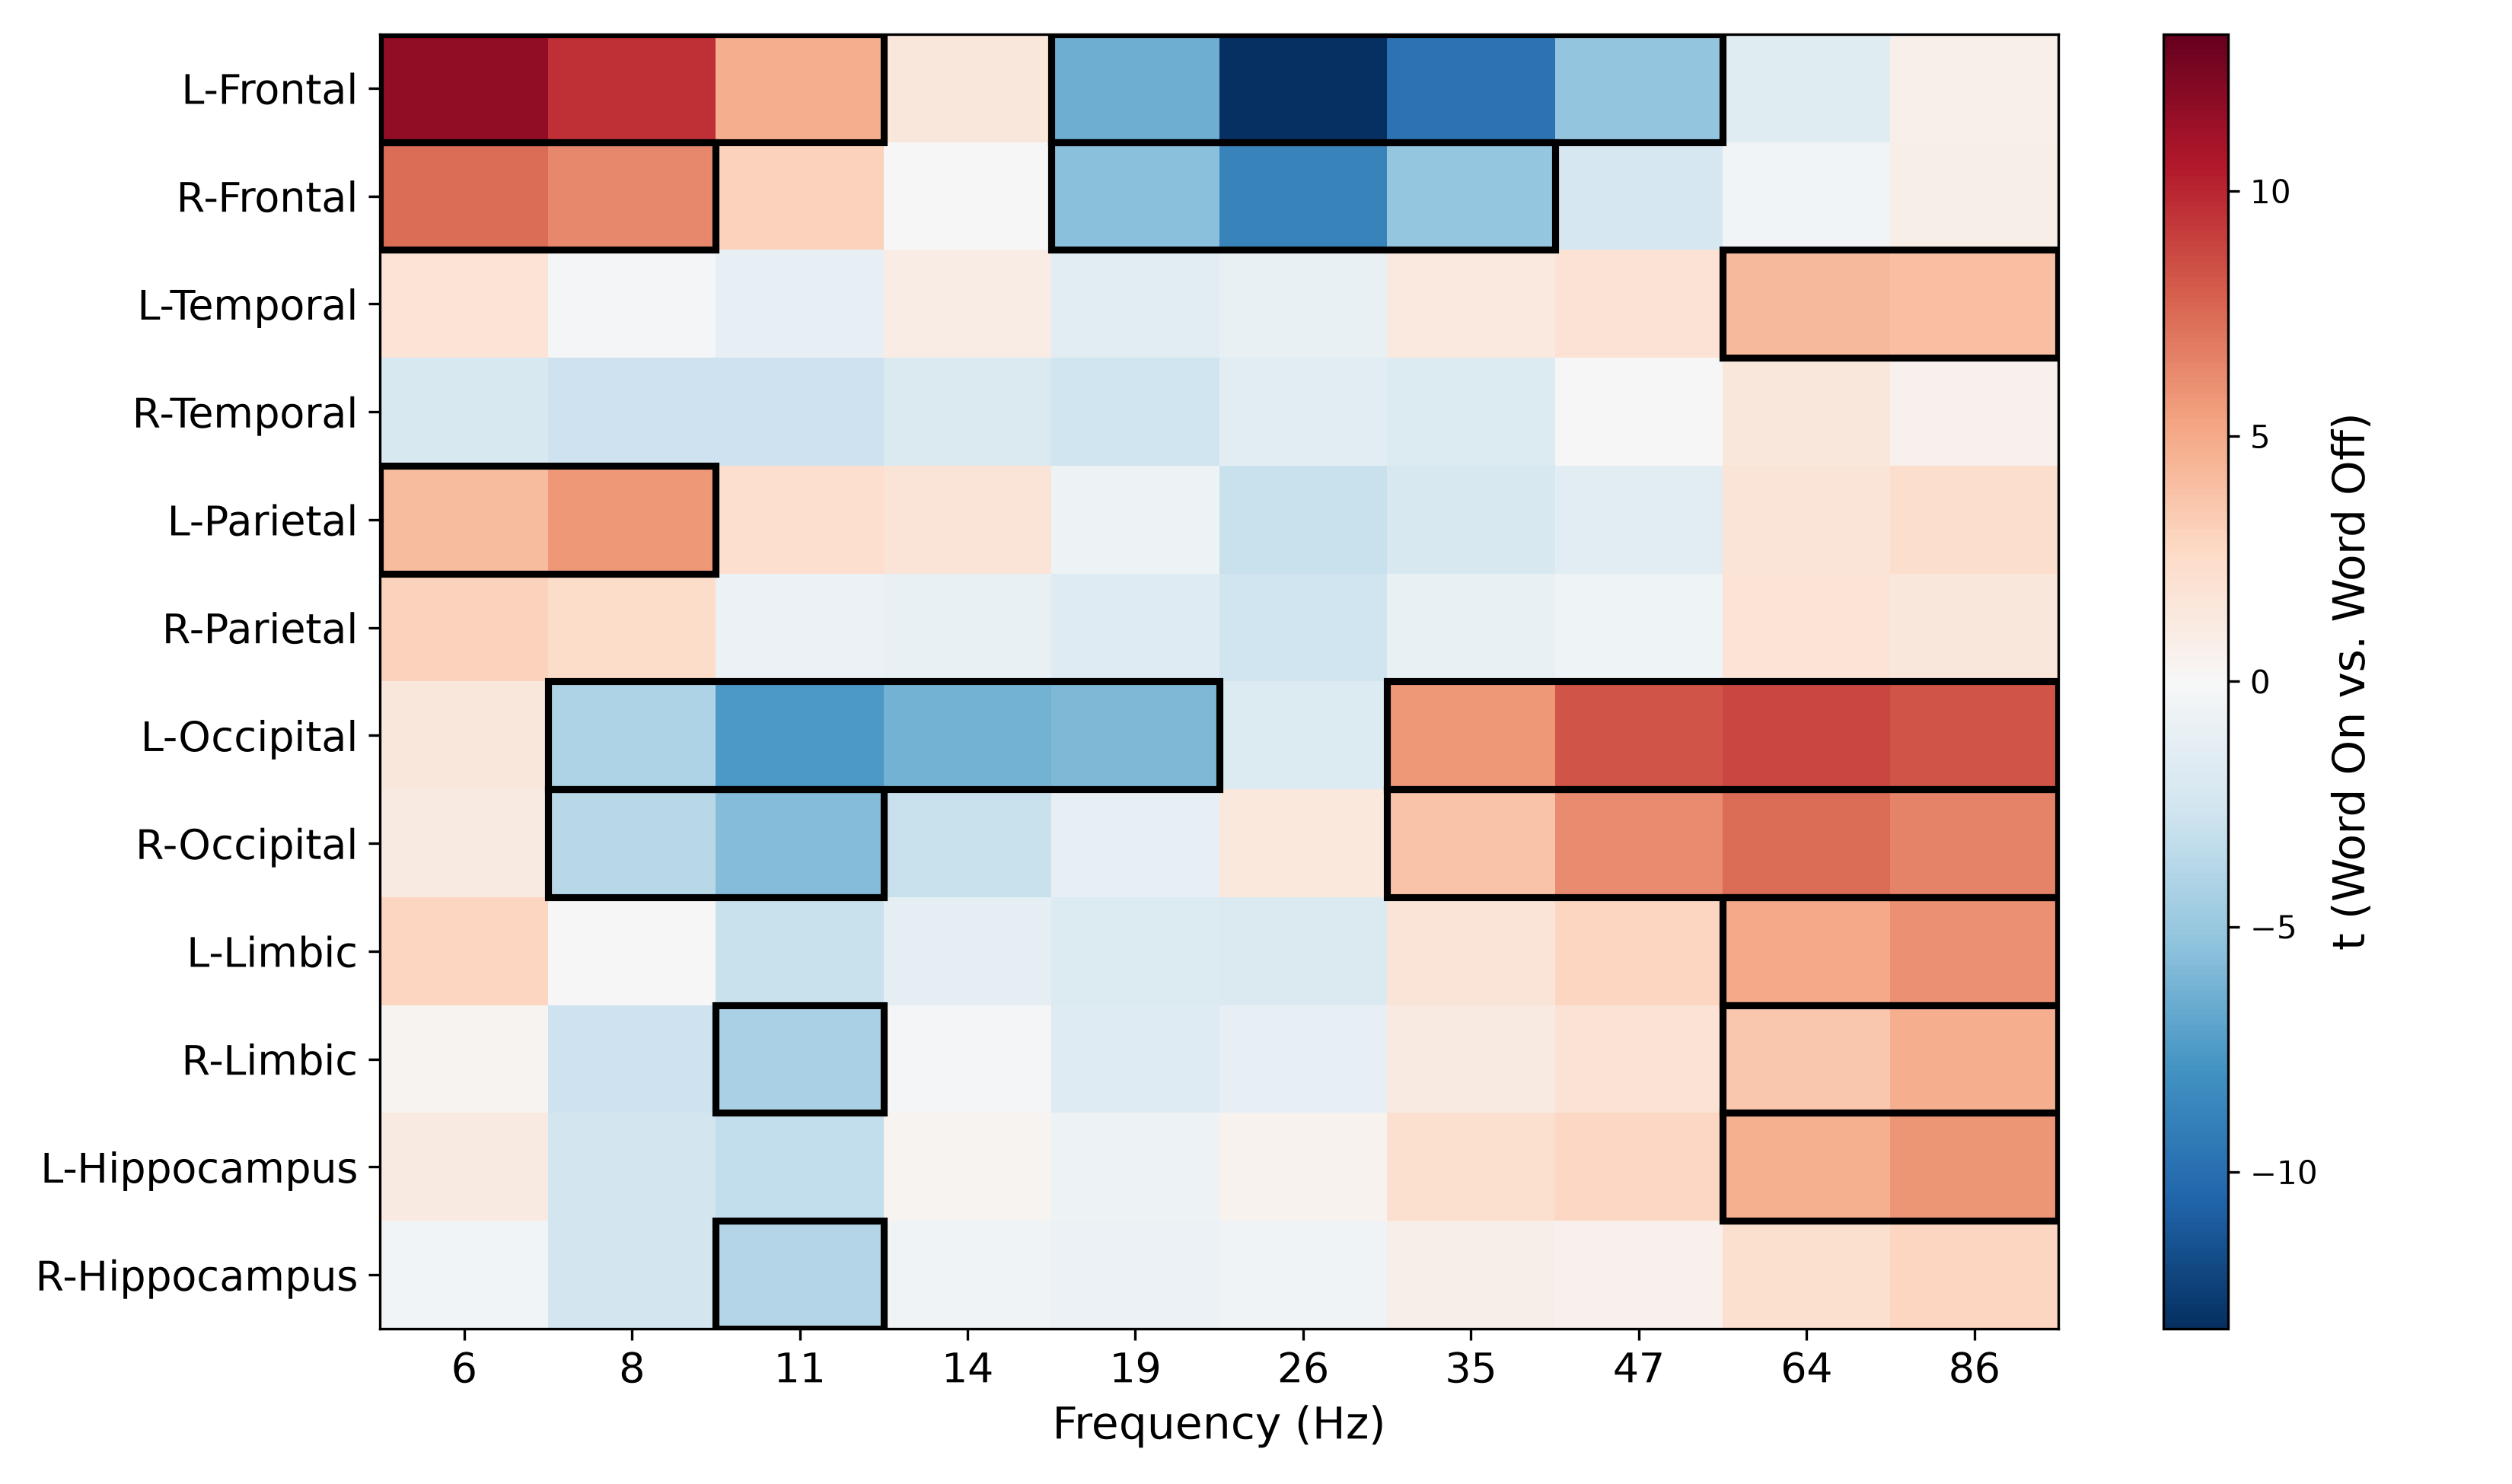
\includegraphics[keepaspectratio,alt={Spectrum
heatmap}]{img/fig2a_spectrum.png}}
\caption{Spectrum heatmap}
\end{figure}

\begin{figure}
\centering
\pandocbounded{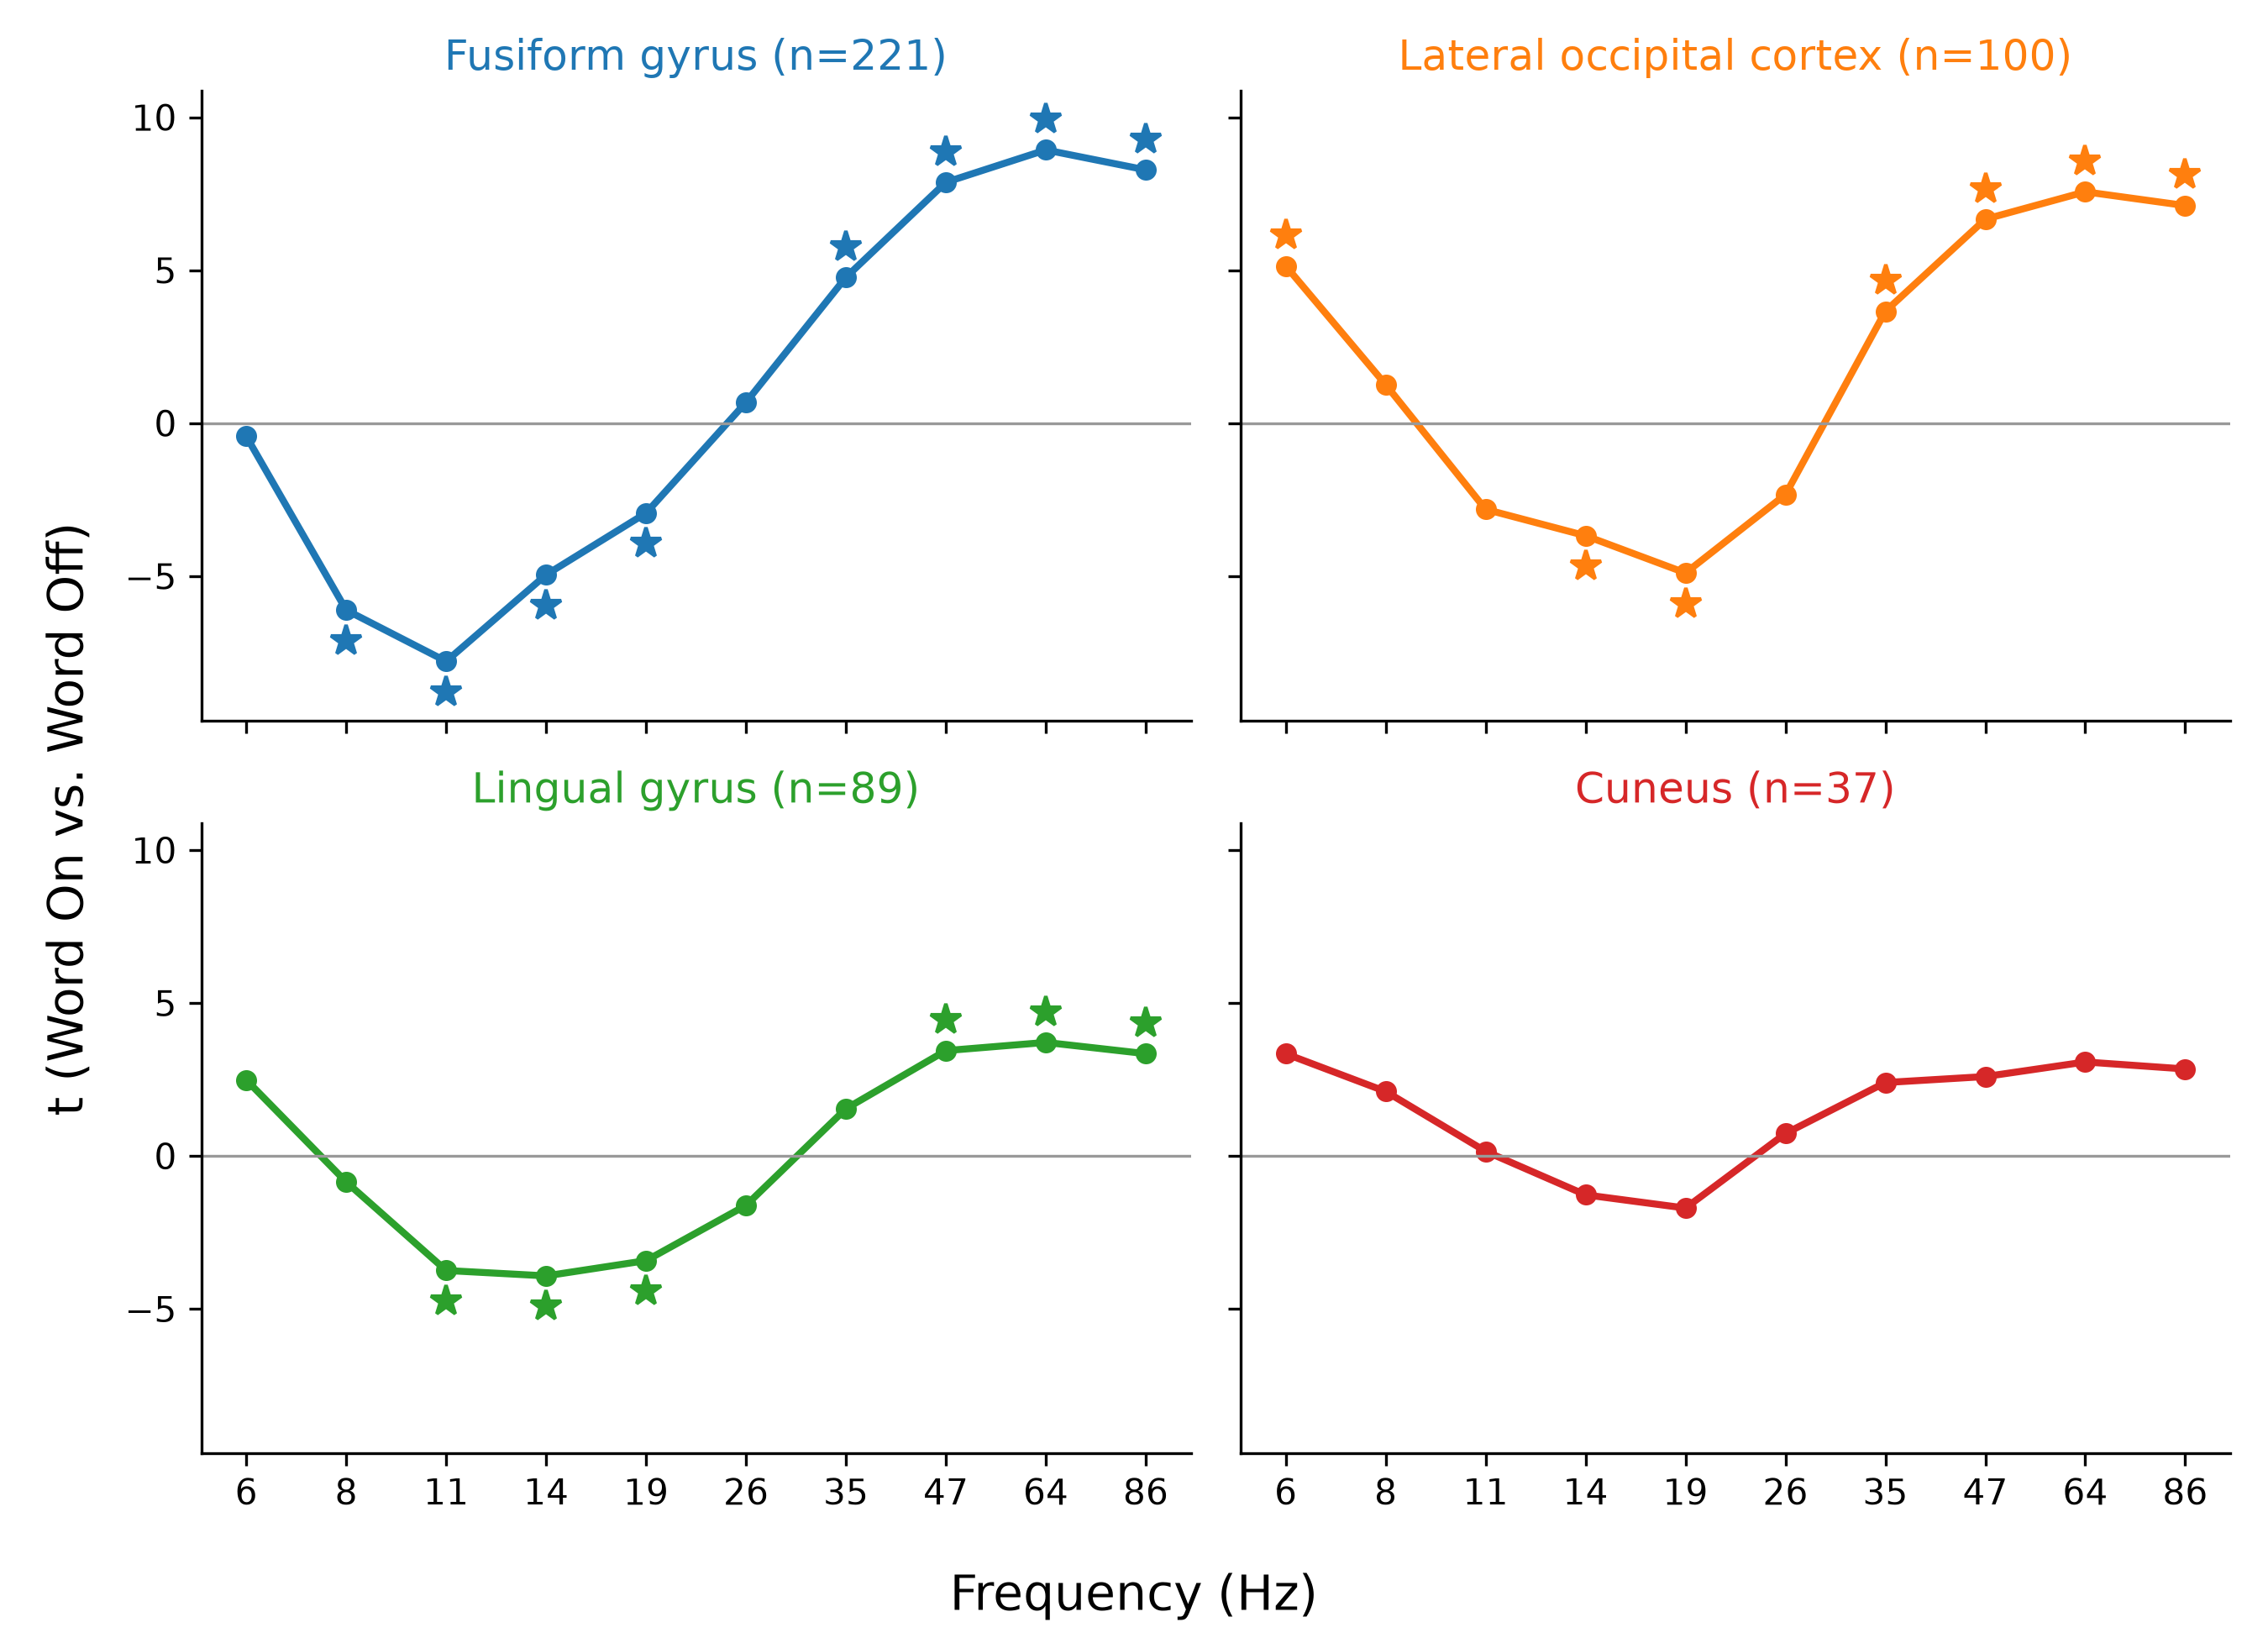
\includegraphics[keepaspectratio,alt={Occipital case
studies}]{img/fig2b_occipital.png}}
\caption{Occipital case studies}
\end{figure}

\begin{itemize}
\tightlist
\item
  Frontal: theta/low-alpha increase (t up to 11) with beta decrease (t
  to −13.5).
\item
  Occipital: alpha--beta decrease (10.6 Hz t $\approx$ −8), broadband increase $\geq$
  35 Hz (t up to 8.6).
\item
  Limbic / hippocampus: mild alpha decrease, gamma increase.
\item
  Occipital subregions (hemispheres pooled; the 4 with most subjects):
  fusiform (199), lateral occipital (86), lingual (77), cuneus (32).
  All: alpha/beta decrease and gamma increase ($\geq$35--47 Hz); fusiform
  strongest (t $\approx$ −7.5 at 11 Hz, +8.9 at 64 Hz); lateral occipital also a
  6 Hz increase; cuneus weakest (gamma only). TFCE, family-wise p
  \textless{} .05. (Smith \& Nichols 2009; Mensen \& Khatami 2013;
  Nichols \& Holmes 2002) \#\#\#\# Mixed model (lobe × band)
\end{itemize}

\begin{figure}
\centering
\pandocbounded{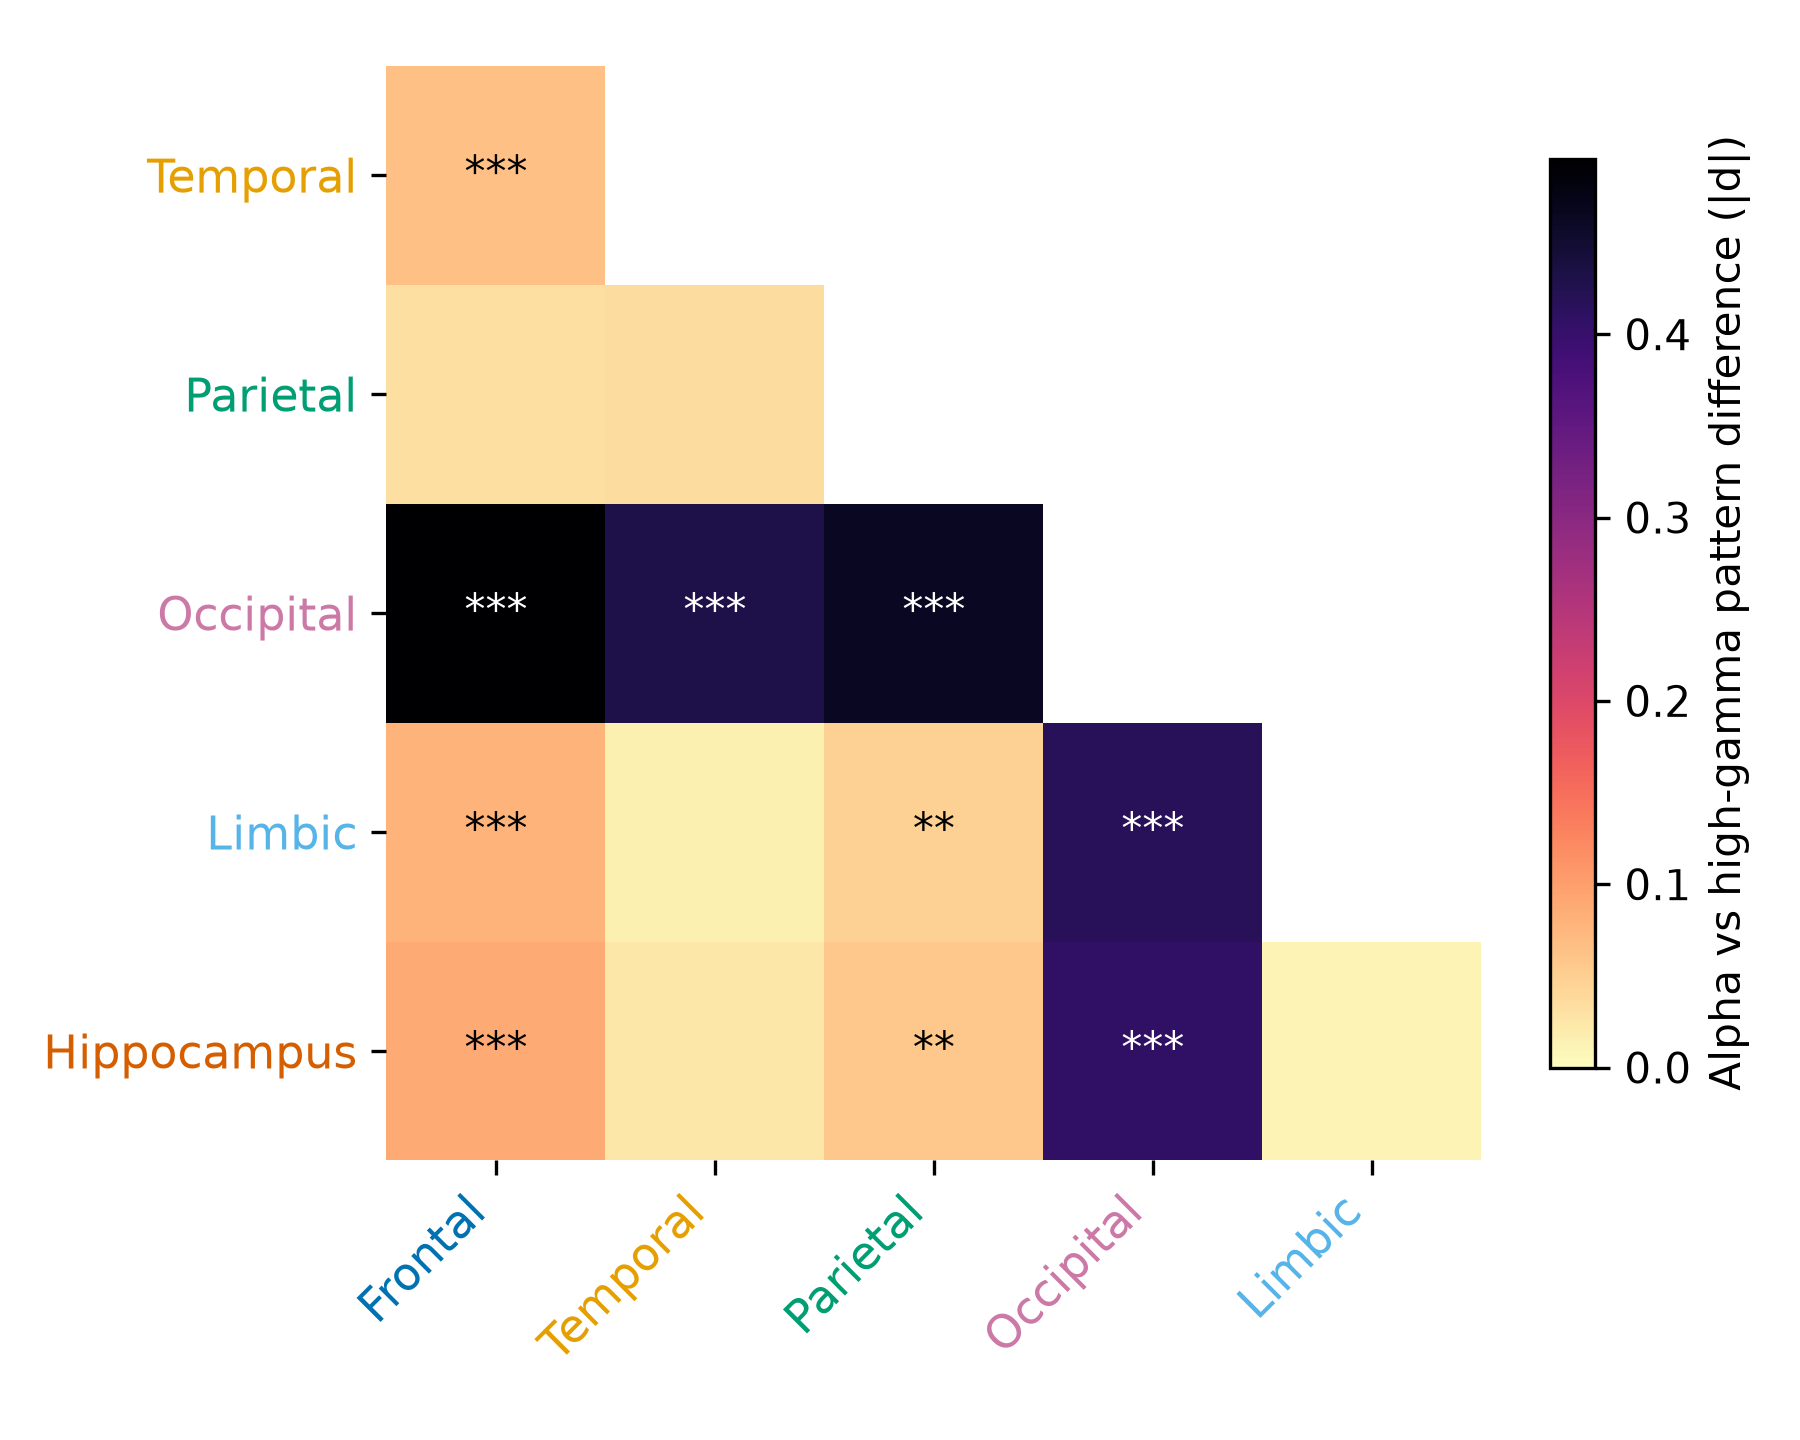
\includegraphics[keepaspectratio,alt={Power, mixed
model}]{img/fig1b_power_mixed.png}}
\caption{Power, mixed model}
\end{figure}

\begin{itemize}
\tightlist
\item
  Does the alpha-vs-high-gamma pattern differ between lobes (lobe × band
  interaction)? 11 of 15 pairs differ (Holm).
\item
  Occipital differs from every other lobe (\textbar d\textbar{}
  0.43--0.53); frontal from temporal, limbic and hippocampus
  (0.06--0.10); parietal from limbic and hippocampus; hippocampus from
  temporal.
\item
  Not different: frontal vs parietal, parietal vs temporal, limbic vs
  temporal (p = .07), hippocampus vs limbic.
\end{itemize}

\subsubsection{2. Order of activation}\label{order-of-activation}

\begin{figure}
\centering
\pandocbounded{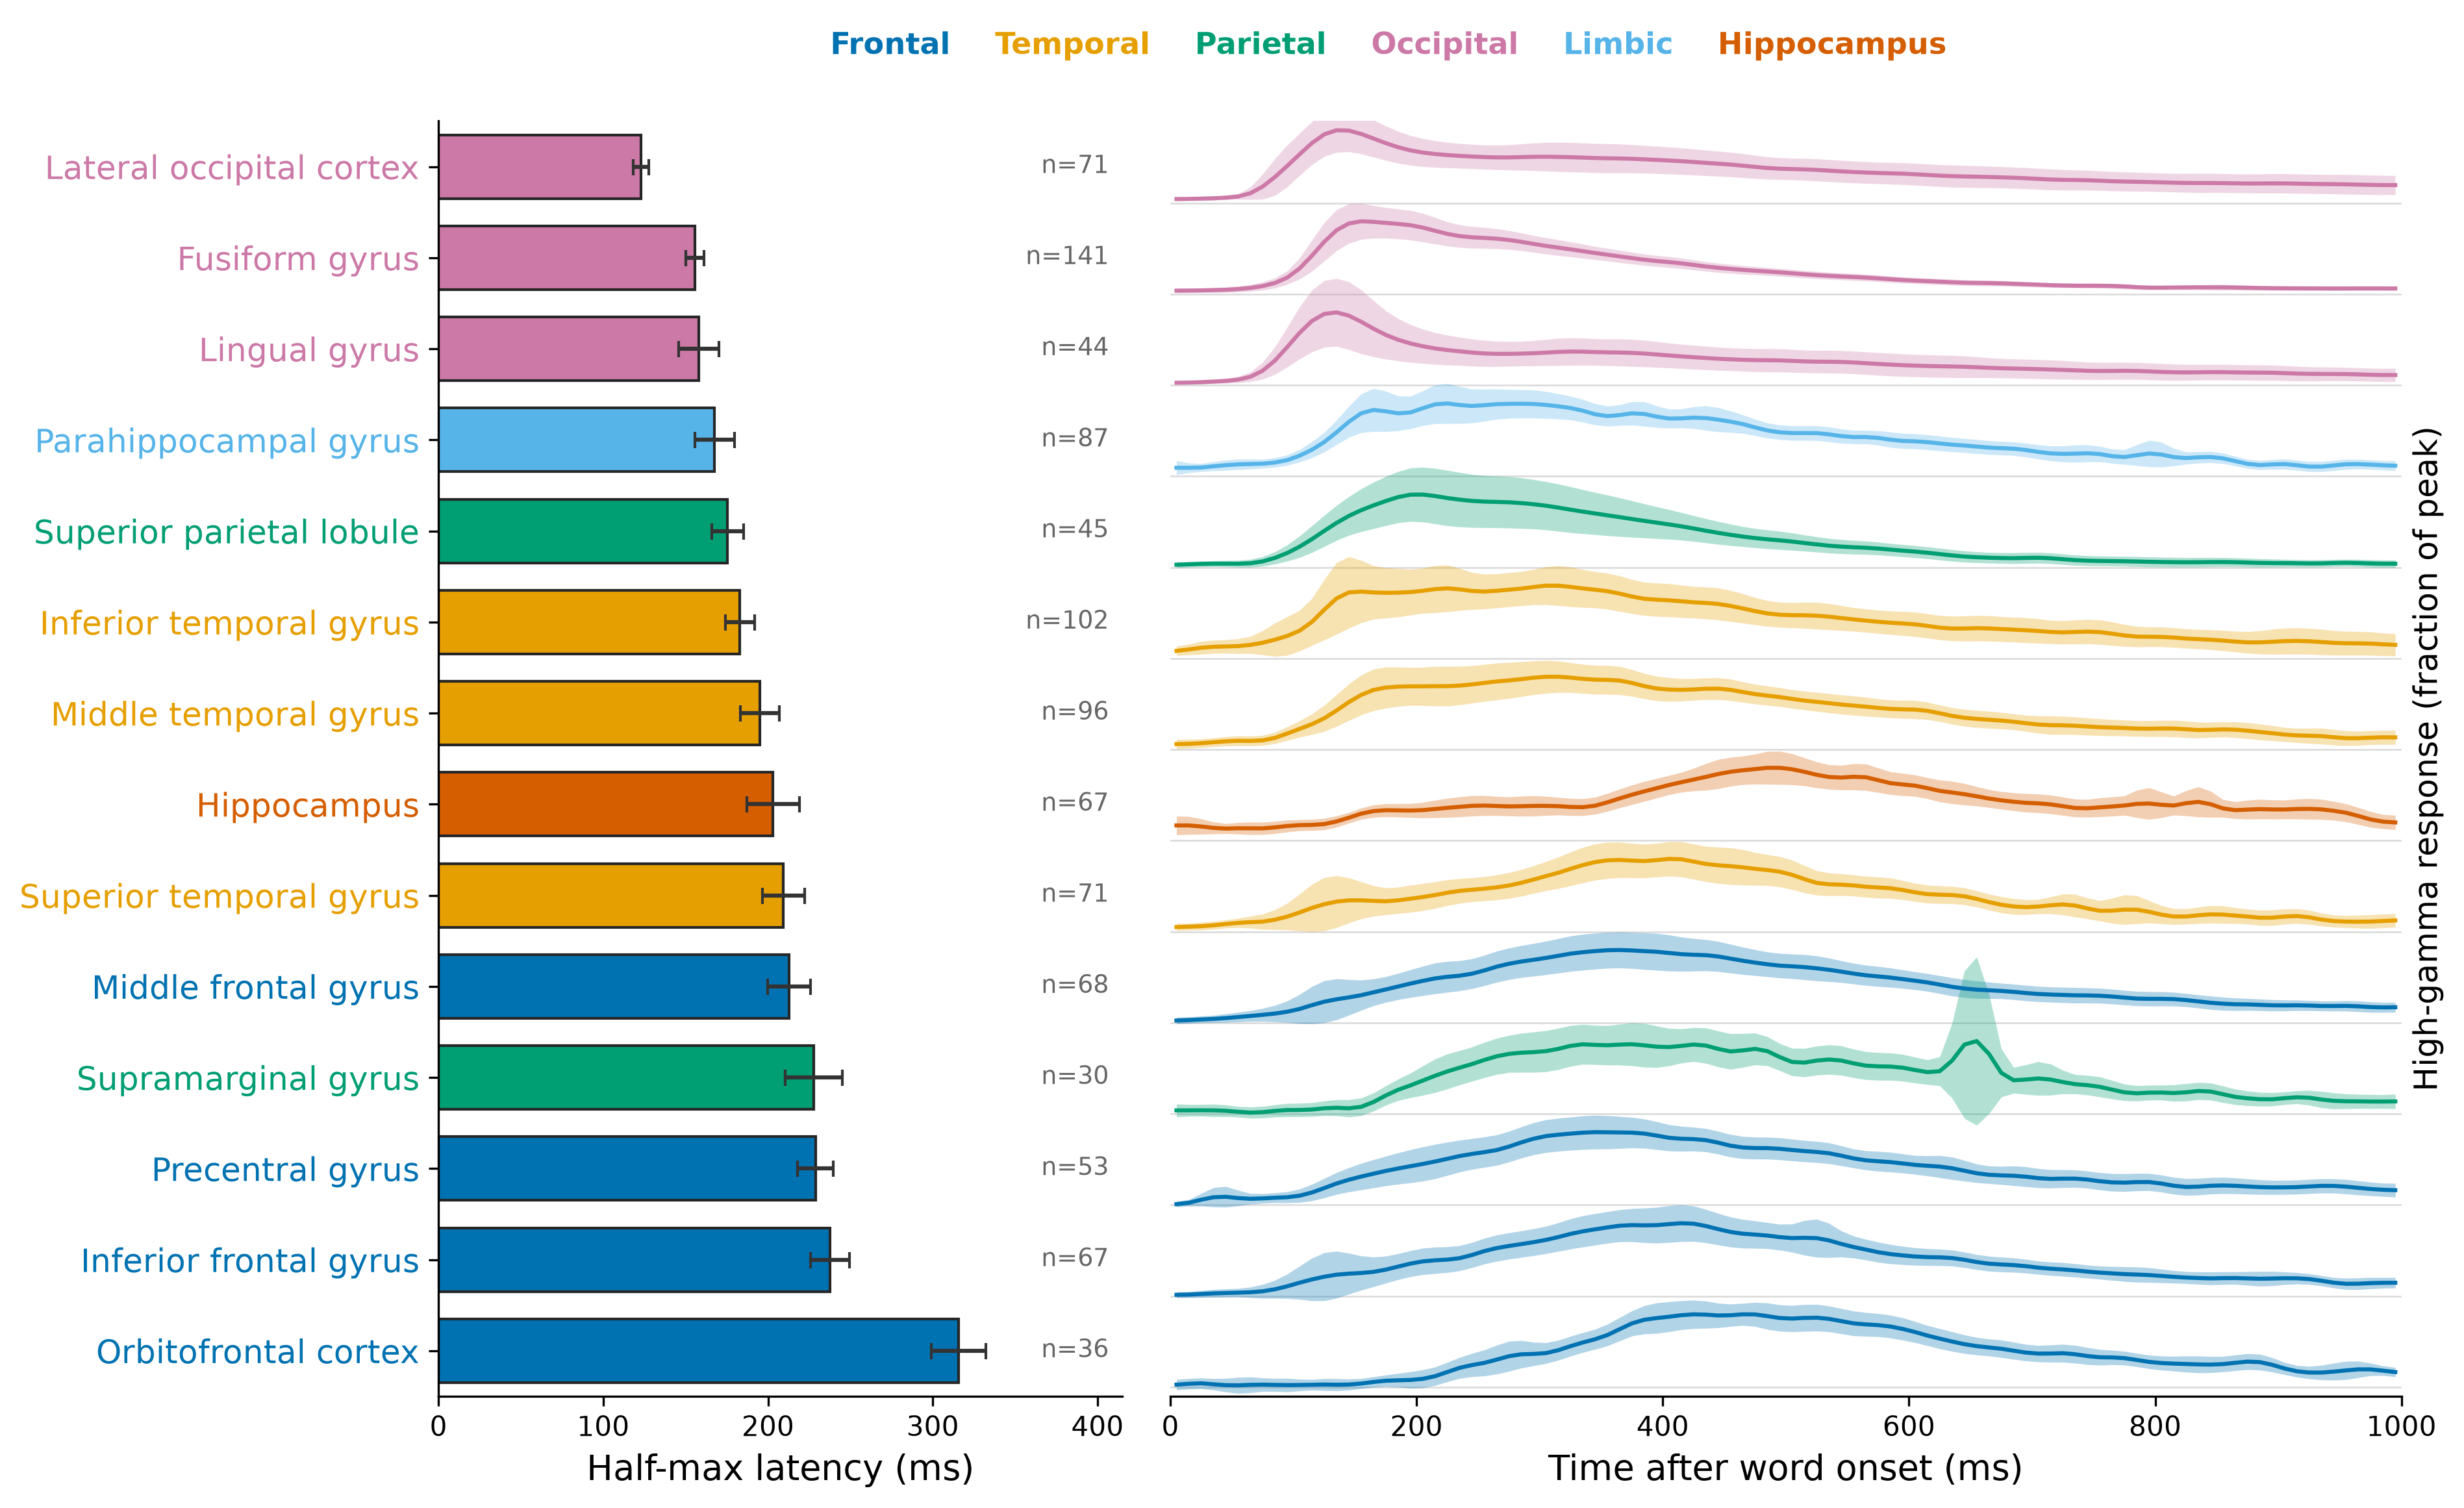
\includegraphics[keepaspectratio,alt={Latency,
subregions}]{img/fig4b_latency_fine.png}}
\caption{Latency, subregions}
\end{figure}

\begin{itemize}
\tightlist
\item
  Posterior → anterior: R occipital 128 ms, L occipital 157 → limbic, R
  temporal (\textasciitilde164--169) → R hippocampus, R parietal
  (\textasciitilde175--178) → L temporal 199, L hippocampus 207, R
  frontal 216 → L parietal 235, L frontal 259 ms.
\item
  Subregions: lateral occipital 122 → lingual 150, fusiform 157 →
  parahippocampal 167, amygdala 170, insula 174 → superior parietal 188,
  temporal gyri \textasciitilde189--194, hippocampus 192 → supramarginal
  214, frontal gyri 215--237 → orbitofrontal 300 ms.
\item
  Early regions: sharp peak \textasciitilde150 ms; hippocampus / insula
  / frontal: broad peaks \textasciitilde350--550 ms.
\end{itemize}

\paragraph{Mixed model (latency per
lobe)}\label{mixed-model-latency-per-lobe}

\begin{figure}
\centering
\pandocbounded{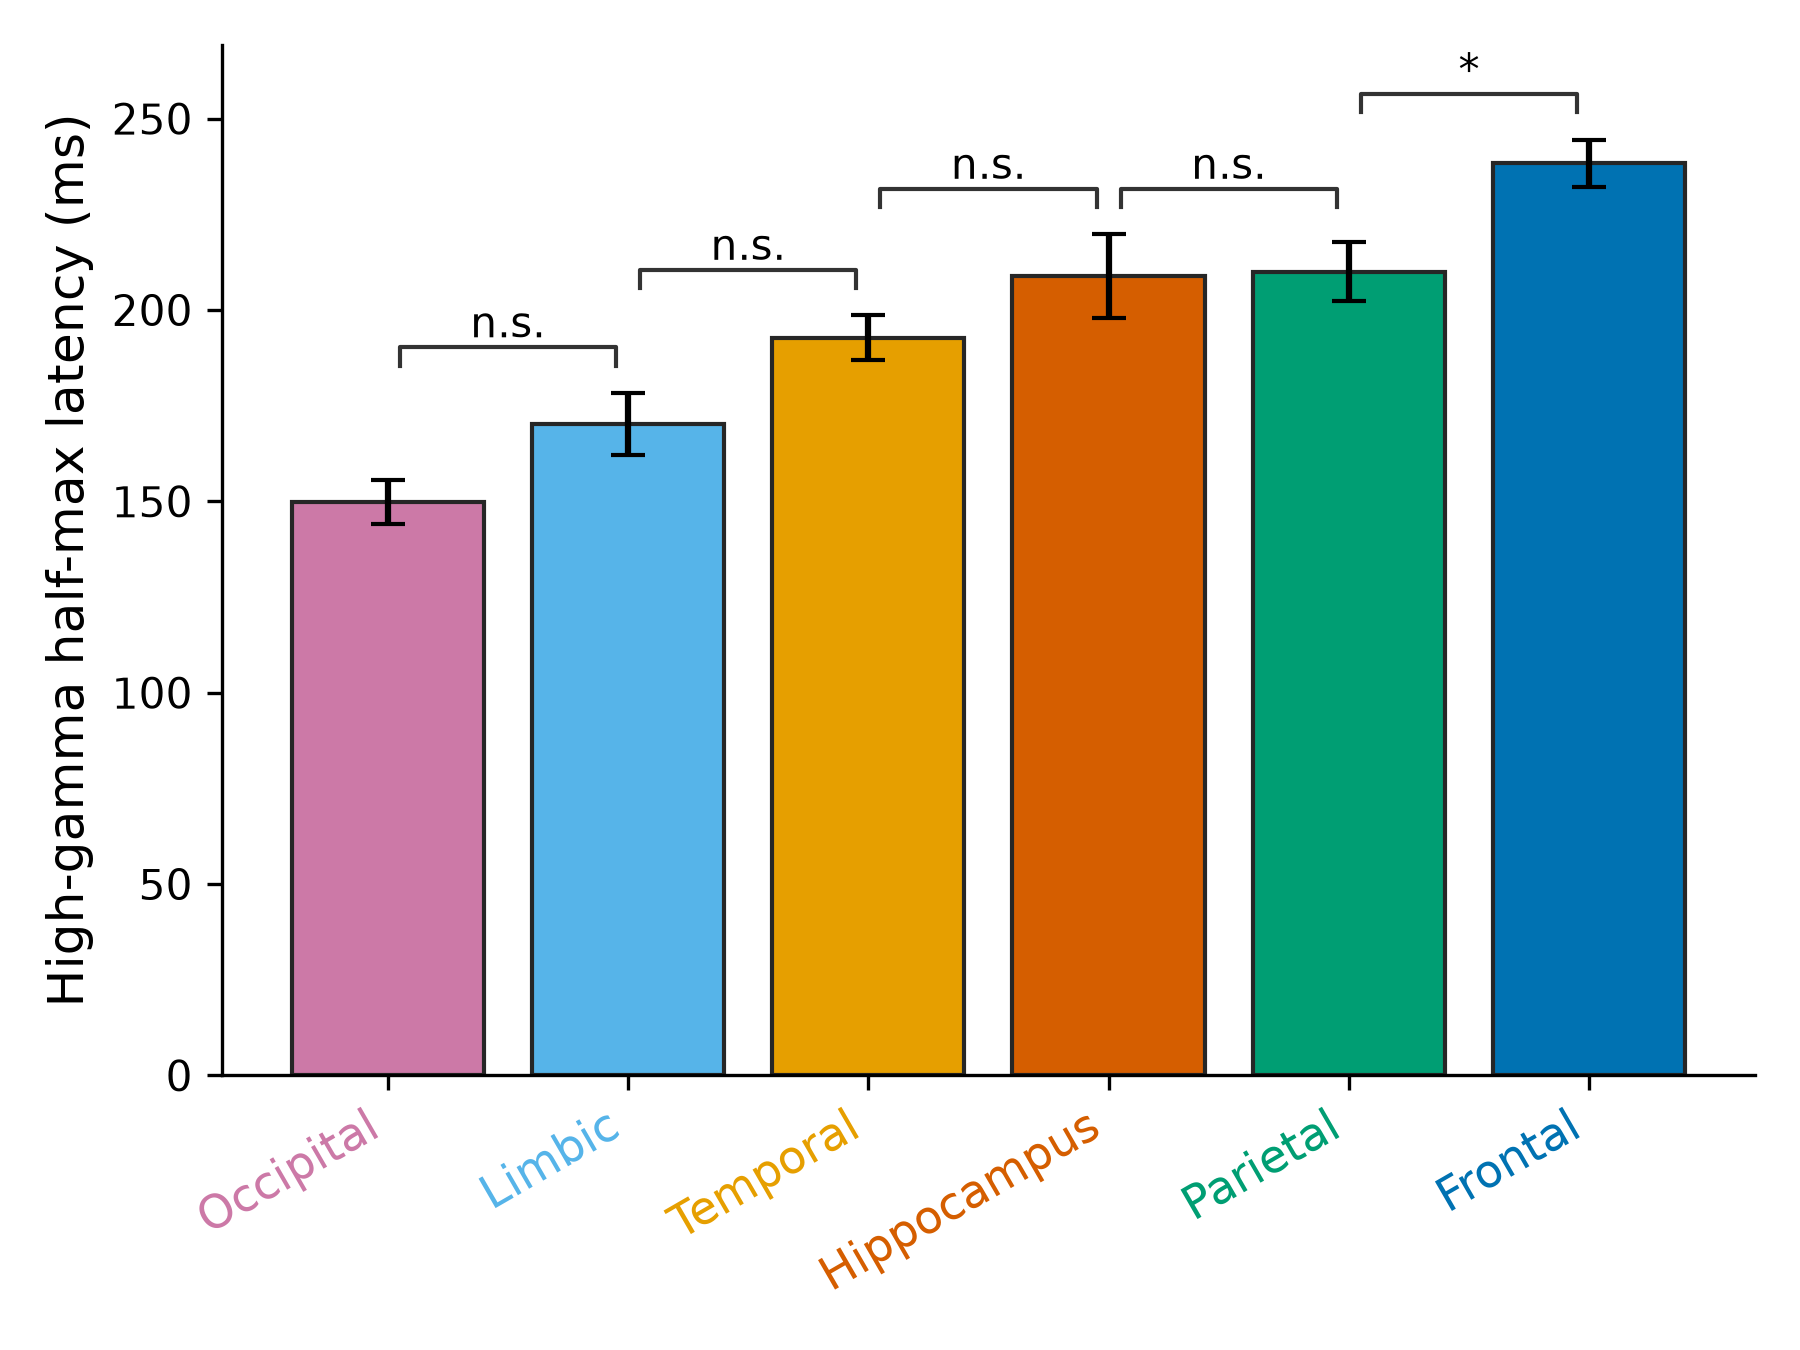
\includegraphics[keepaspectratio,alt={Latency, mixed
model}]{img/fig4c_latency_mixed.png}}
\caption{Latency, mixed model}
\end{figure}

\begin{itemize}
\tightlist
\item
  Estimated latency: occipital 148 → limbic 171 → temporal 190 →
  hippocampus 199 → parietal 215 → frontal 241 ms.
\item
  Neighbouring steps (brackets): occipital \textless{} limbic (p = .045)
  and parietal \textless{} frontal (p = .045); limbic--temporal (p =
  .08), temporal--hippocampus and hippocampus--parietal (p = .39) not
  separable.
\item
  All 15 pairs (CSV): 12 differ (Holm p \textless{} .05); posterior →
  anterior holds at the lobe level, not every step.
\end{itemize}

\subsubsection{3. Synchrony}\label{synchrony-1}

\begin{figure}
\centering
\pandocbounded{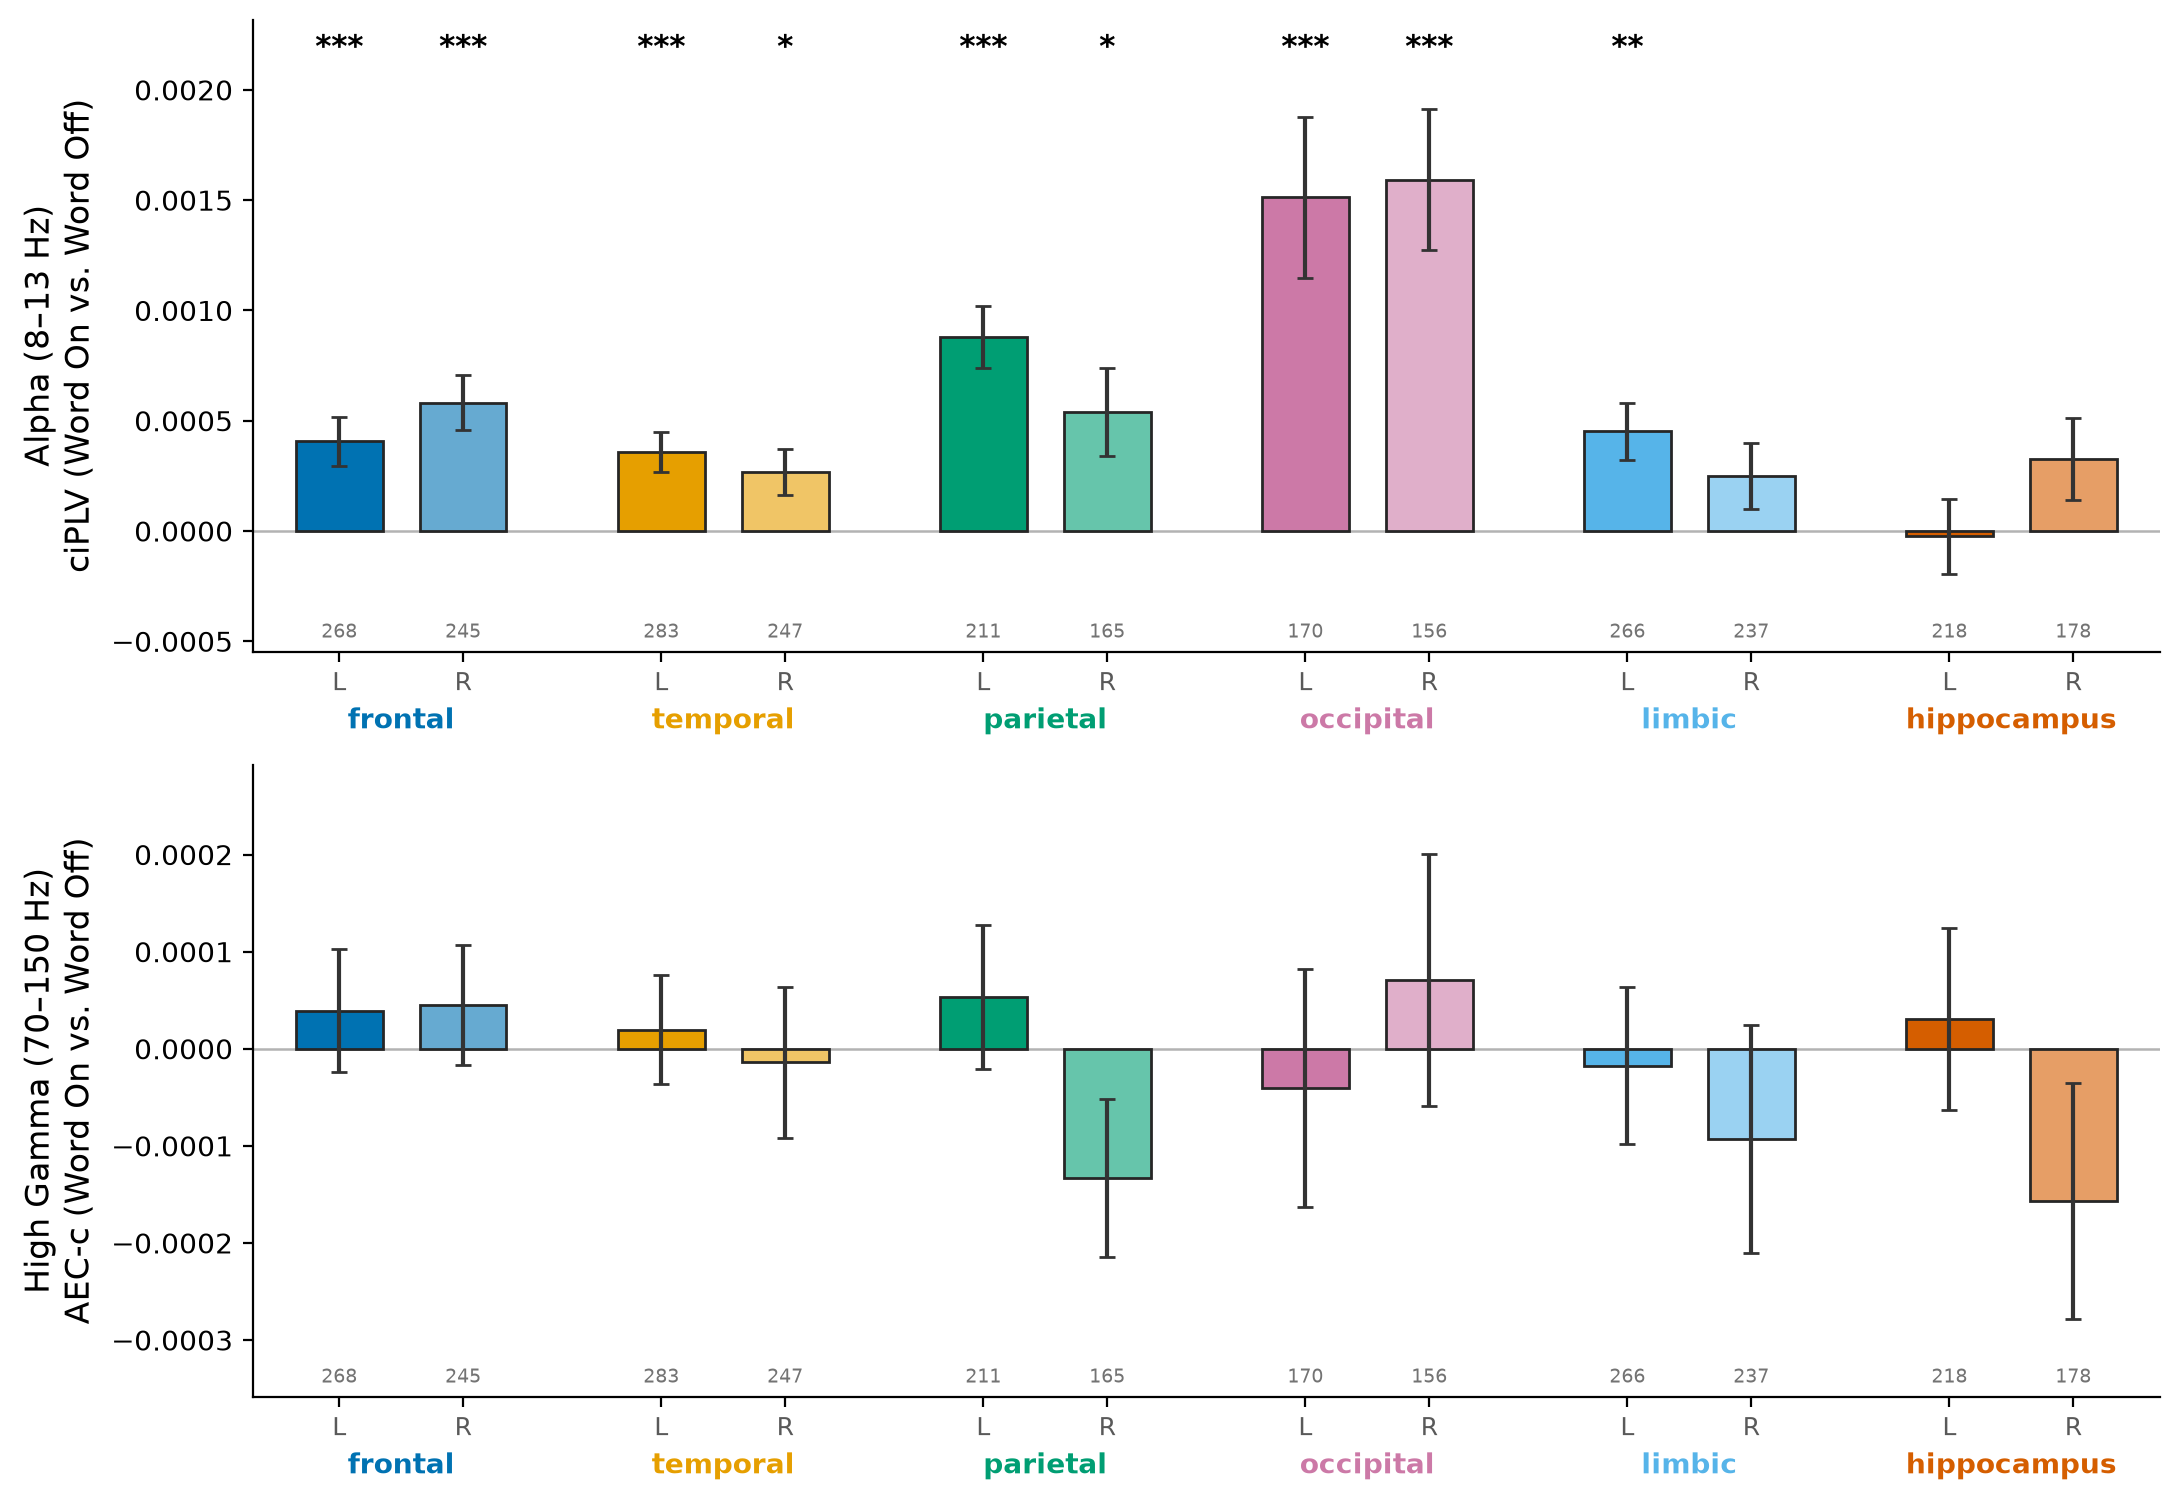
\includegraphics[keepaspectratio,alt={Synchrony per
ROI}]{img/fig5_synchrony.png}}
\caption{Synchrony per ROI}
\end{figure}

\begin{itemize}
\tightlist
\item
  Alpha ciPLV increases in 10 / 12 ROIs, about twice as much in
  occipital (\textasciitilde0.0016) as elsewhere
  (\textasciitilde0.0003--0.0008).
\item
  High-gamma AEC-c: no significant change in any ROI.
\end{itemize}

\paragraph{Time-resolved network}\label{time-resolved-network}

\begin{figure}
\centering
\pandocbounded{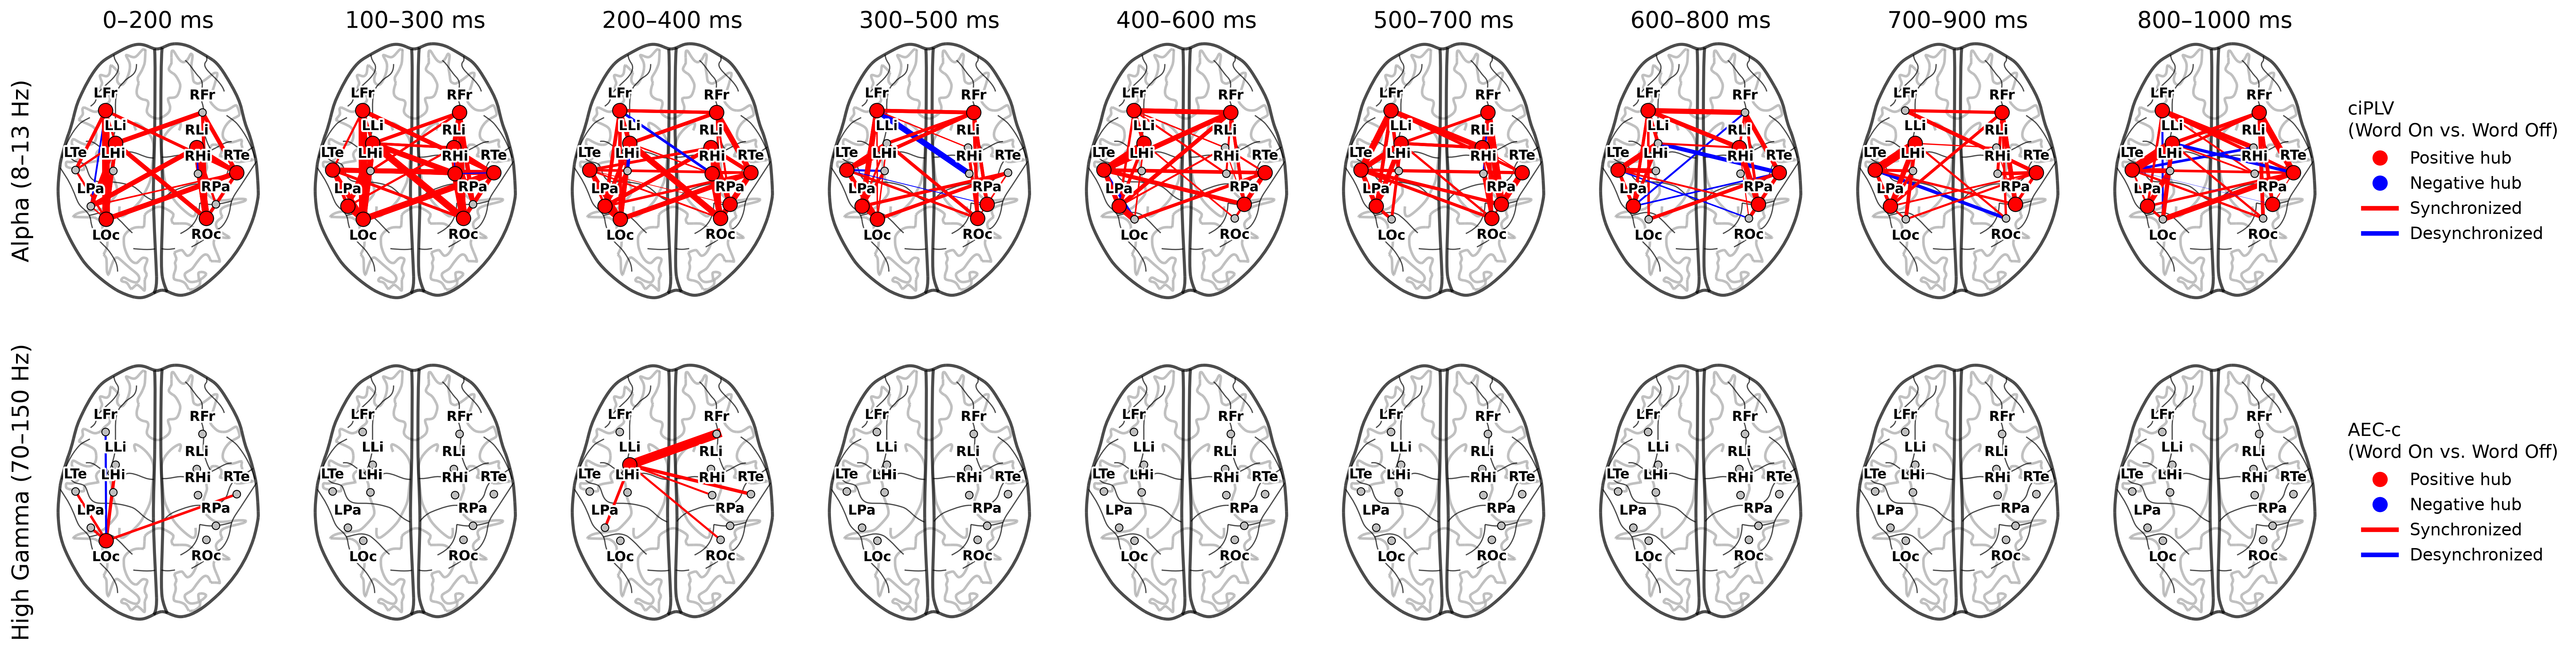
\includegraphics[keepaspectratio,alt={Epoch
network}]{img/fig6a_epochs.png}}
\caption{Epoch network}
\end{figure}

\begin{itemize}
\tightlist
\item
  Alpha: 38 hub × epoch cells; occipital hubs 0--400 ms; parietal from
  100 ms; frontal, temporal, limbic mainly 400--1000 ms; fine regions (9
  cells): L fusiform 0--400 ms → L inferior/middle temporal 500--1000
  ms, L orbitofrontal 400--600 ms.
\item
  High gamma: 3 hubs (bilateral occipital 0--200 ms, L limbic 200--400
  ms); no fine-region hubs; no late desynchronization.
\end{itemize}

\subsubsection{4. Anticipation (blank length before the
word)}\label{anticipation-blank-length-before-the-word}

\begin{figure}
\centering
\pandocbounded{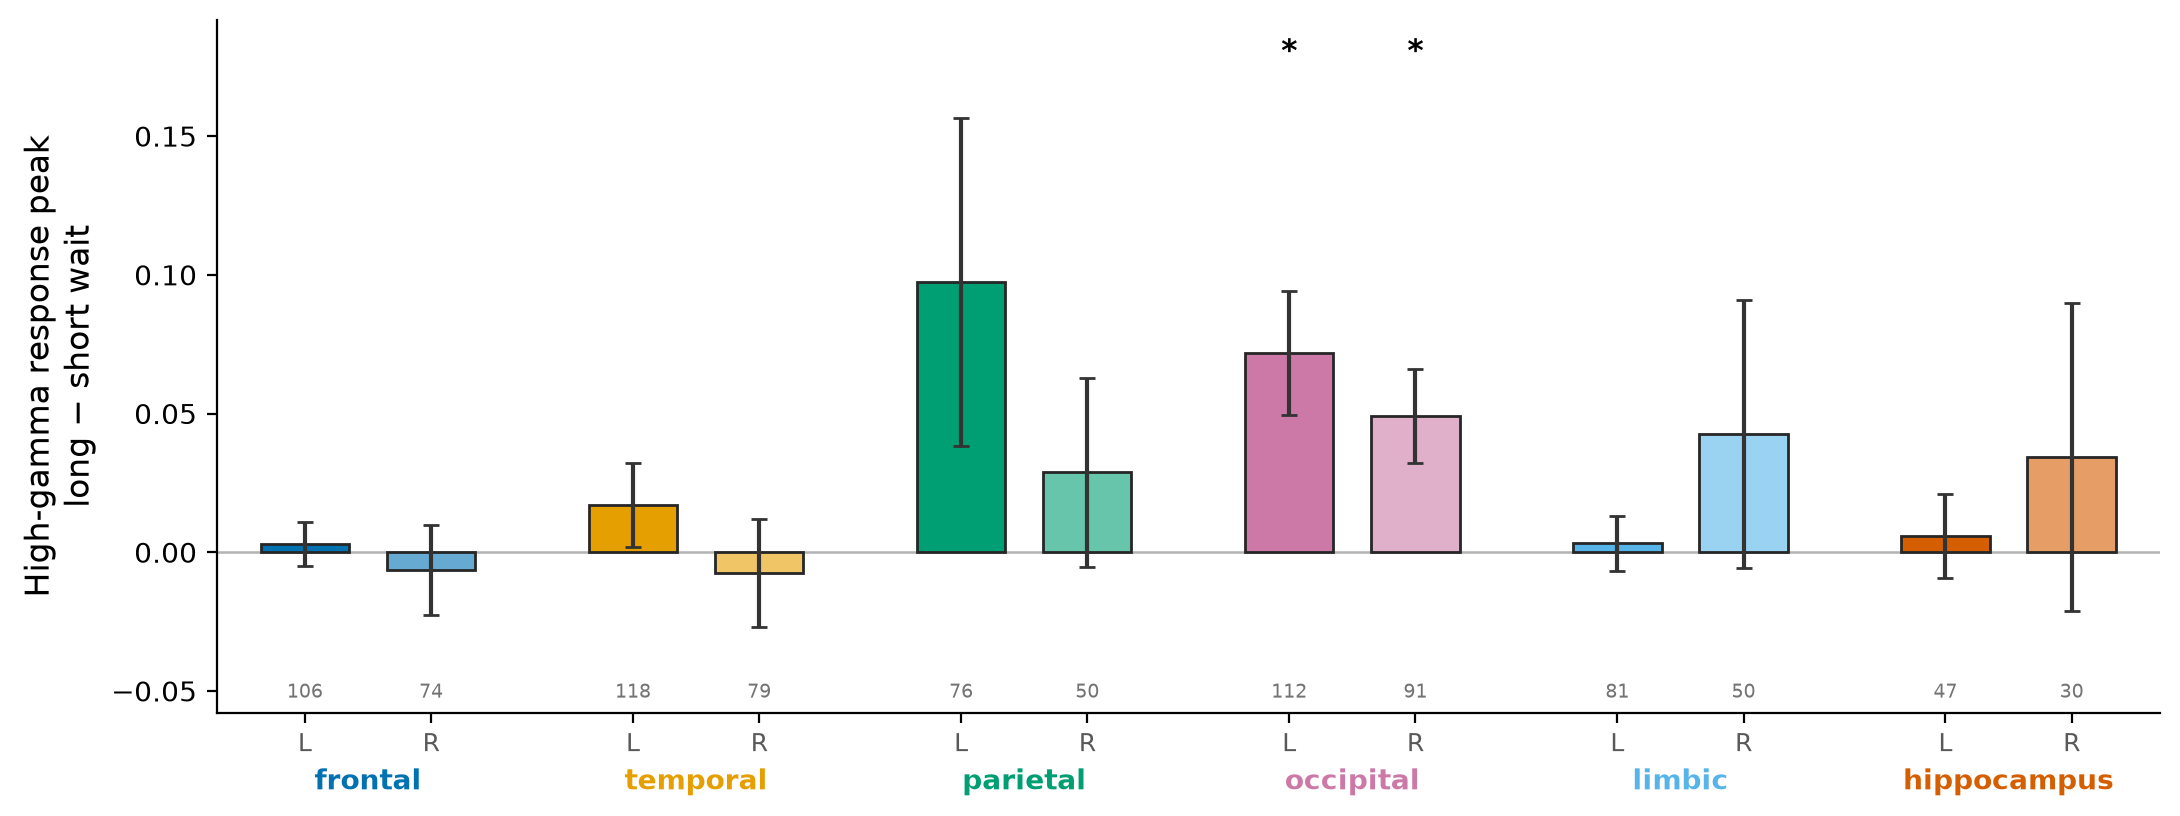
\includegraphics[keepaspectratio,alt={Anticipation}]{img/fig9_anticipation.png}}
\caption{Anticipation}
\end{figure}

\begin{itemize}
\tightlist
\item
  Occipital high-gamma peak larger after long than short waits (L
  +0.078, R +0.053; q = .024 both); no other ROI significant.
\item
  Consistent with temporal expectation boosting visual responses (Lima
  et al.~2011, monkey V1; Nobre \& van Ede 2018), but a shorter blank
  also leaves less time for the previous word's offset response to decay
  (baseline).
\end{itemize}

\subsubsection{5. Recall prediction over the response (encoding
contrast)}\label{recall-prediction-over-the-response-encoding-contrast}

\begin{figure}
\centering
\pandocbounded{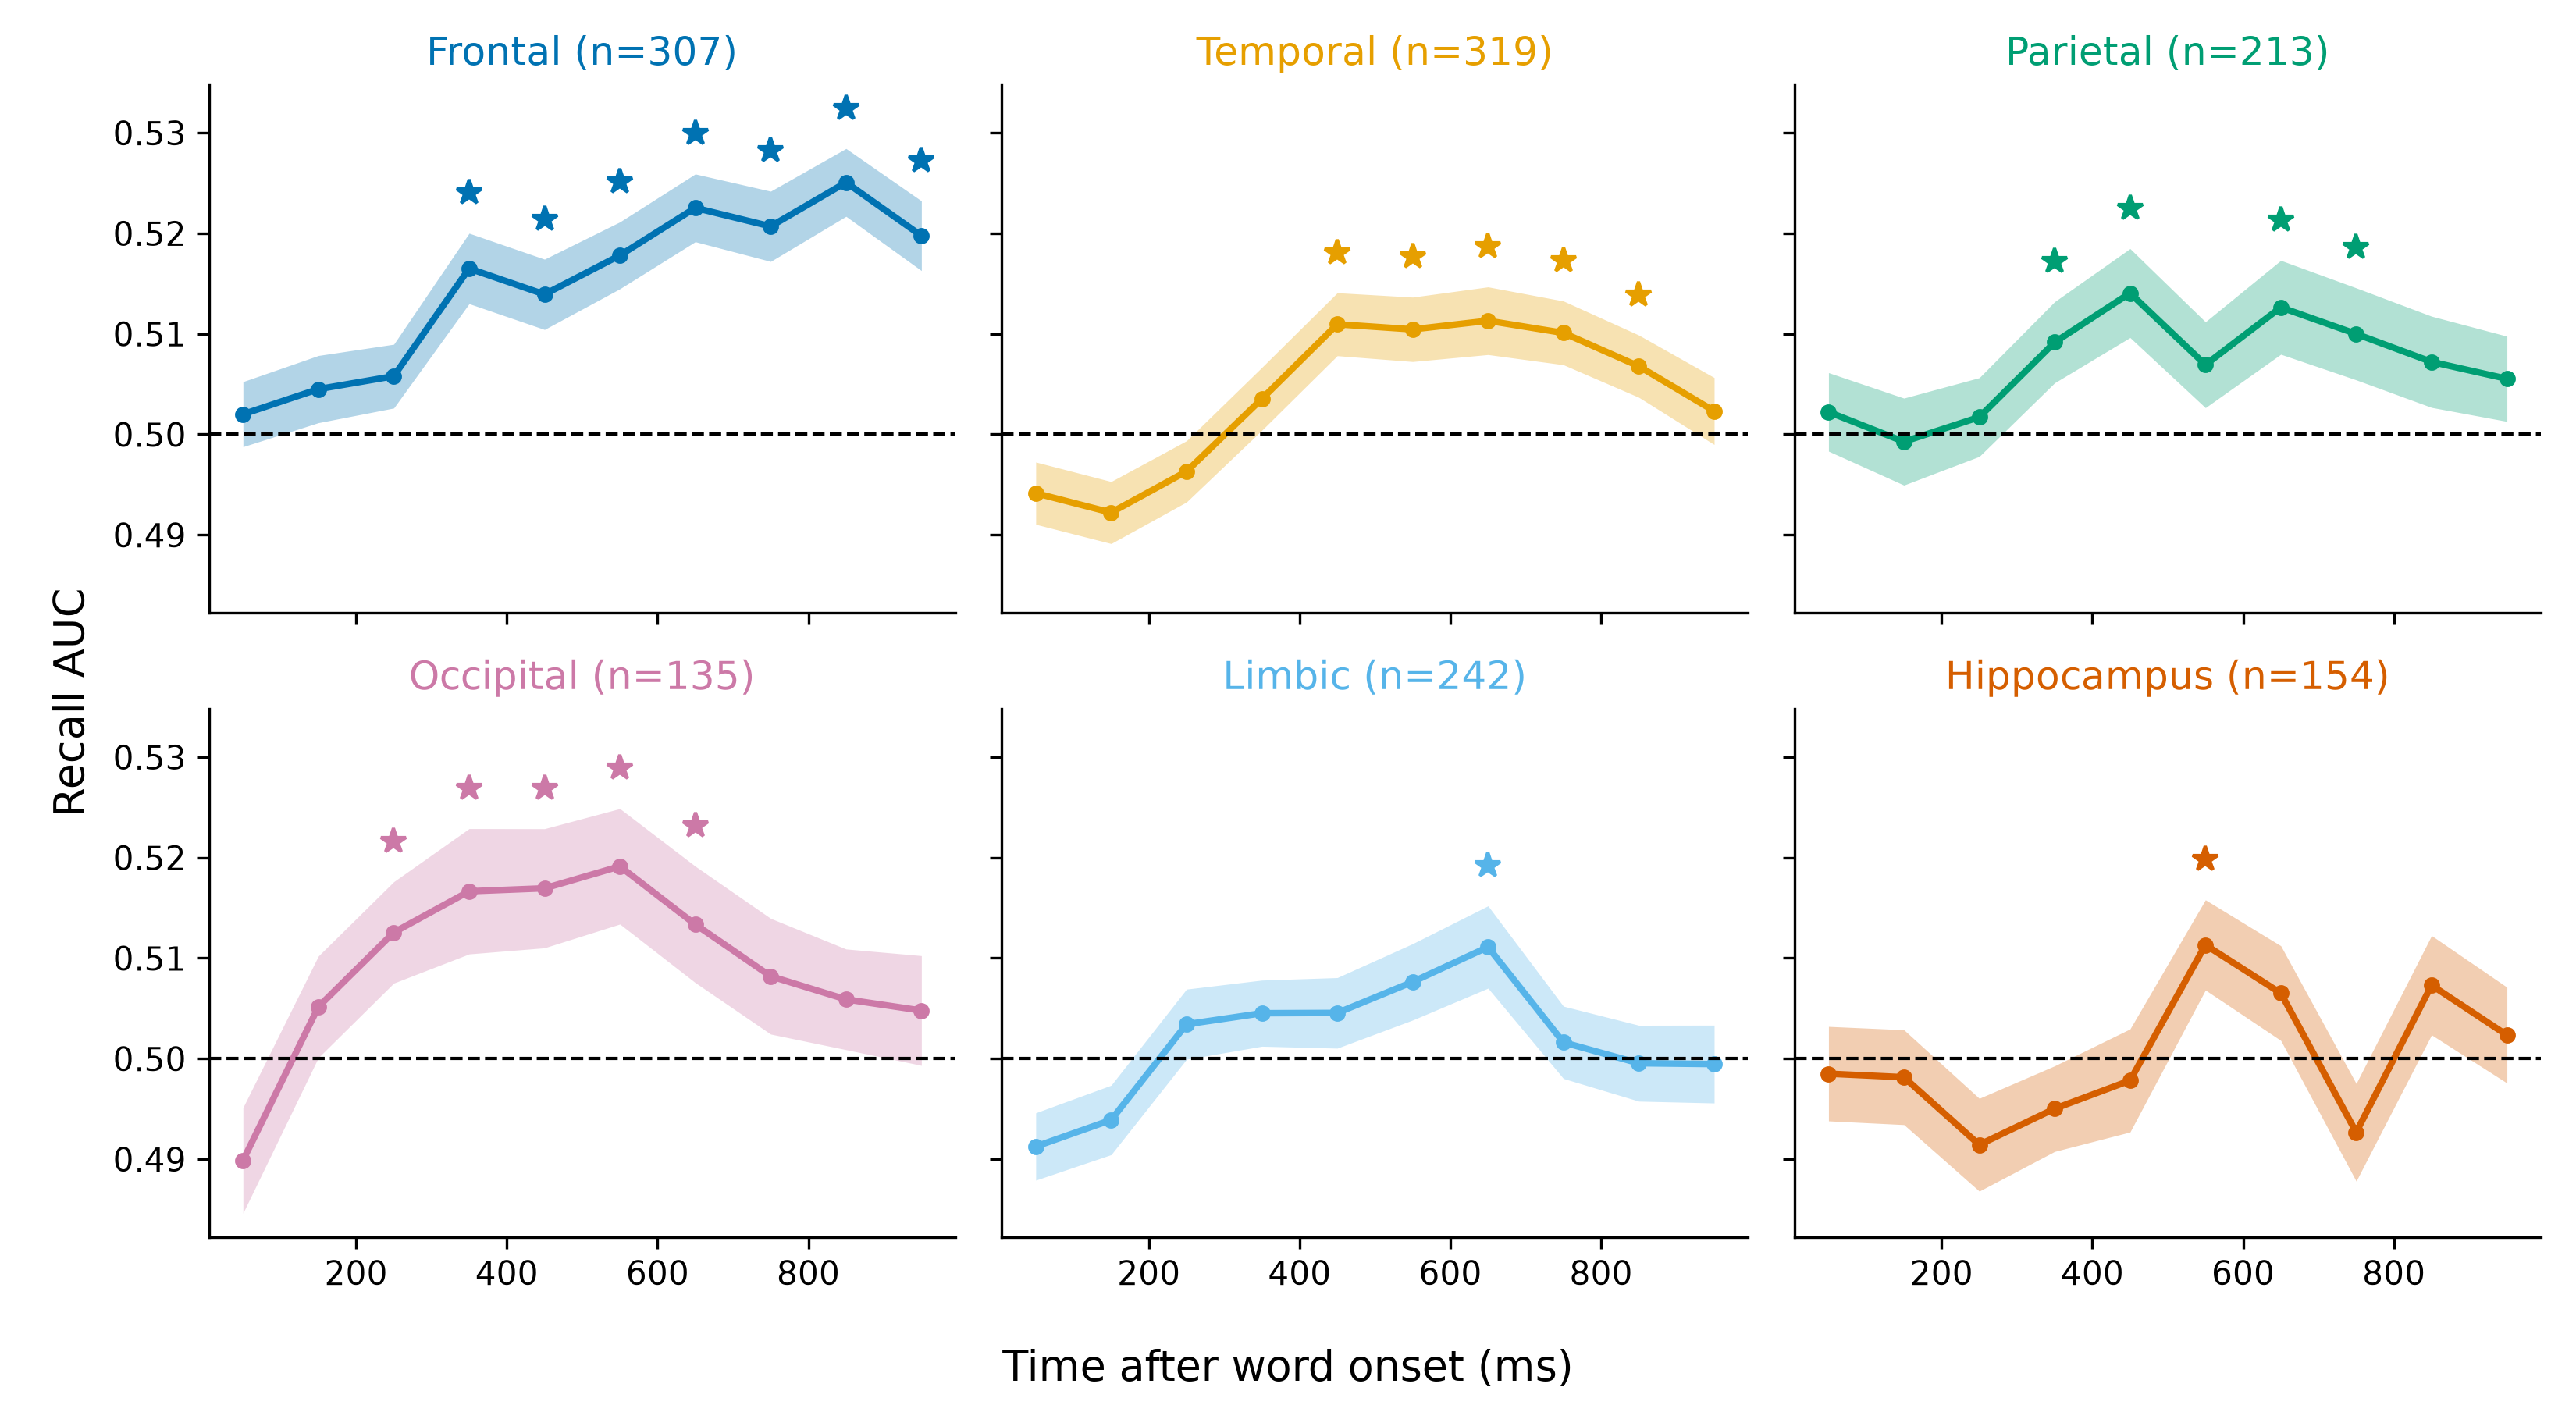
\includegraphics[keepaspectratio,alt={Recall decoding
over time}]{img/fig7_recall_time.png}}
\caption{Recall decoding over time}
\end{figure}

\begin{itemize}
\tightlist
\item
  No lobe predicts recall before 200--300 ms (first significant window:
  frontal and occipital 200--300 ms).
\item
  Frontal: sustained 200--1000 ms, highest at 800--900 ms (AUC 0.525).
\item
  Occipital: 200--700 ms only (peak 0.521 at 300--400 ms); temporal
  400--900 ms; parietal 300--900 ms (patchy); limbic and hippocampus
  500--700 ms.
\item
  AUCs are low ($\leq$ 0.525) because each classifier uses one lobe's high
  gamma in one window. Same direction as Burke, Long et al.~2014
  (encoding contrast: early posterior, late frontal HFA SME).
\end{itemize}

\subsubsection{6. Reliability across
sessions}\label{reliability-across-sessions}

\begin{figure}
\centering
\pandocbounded{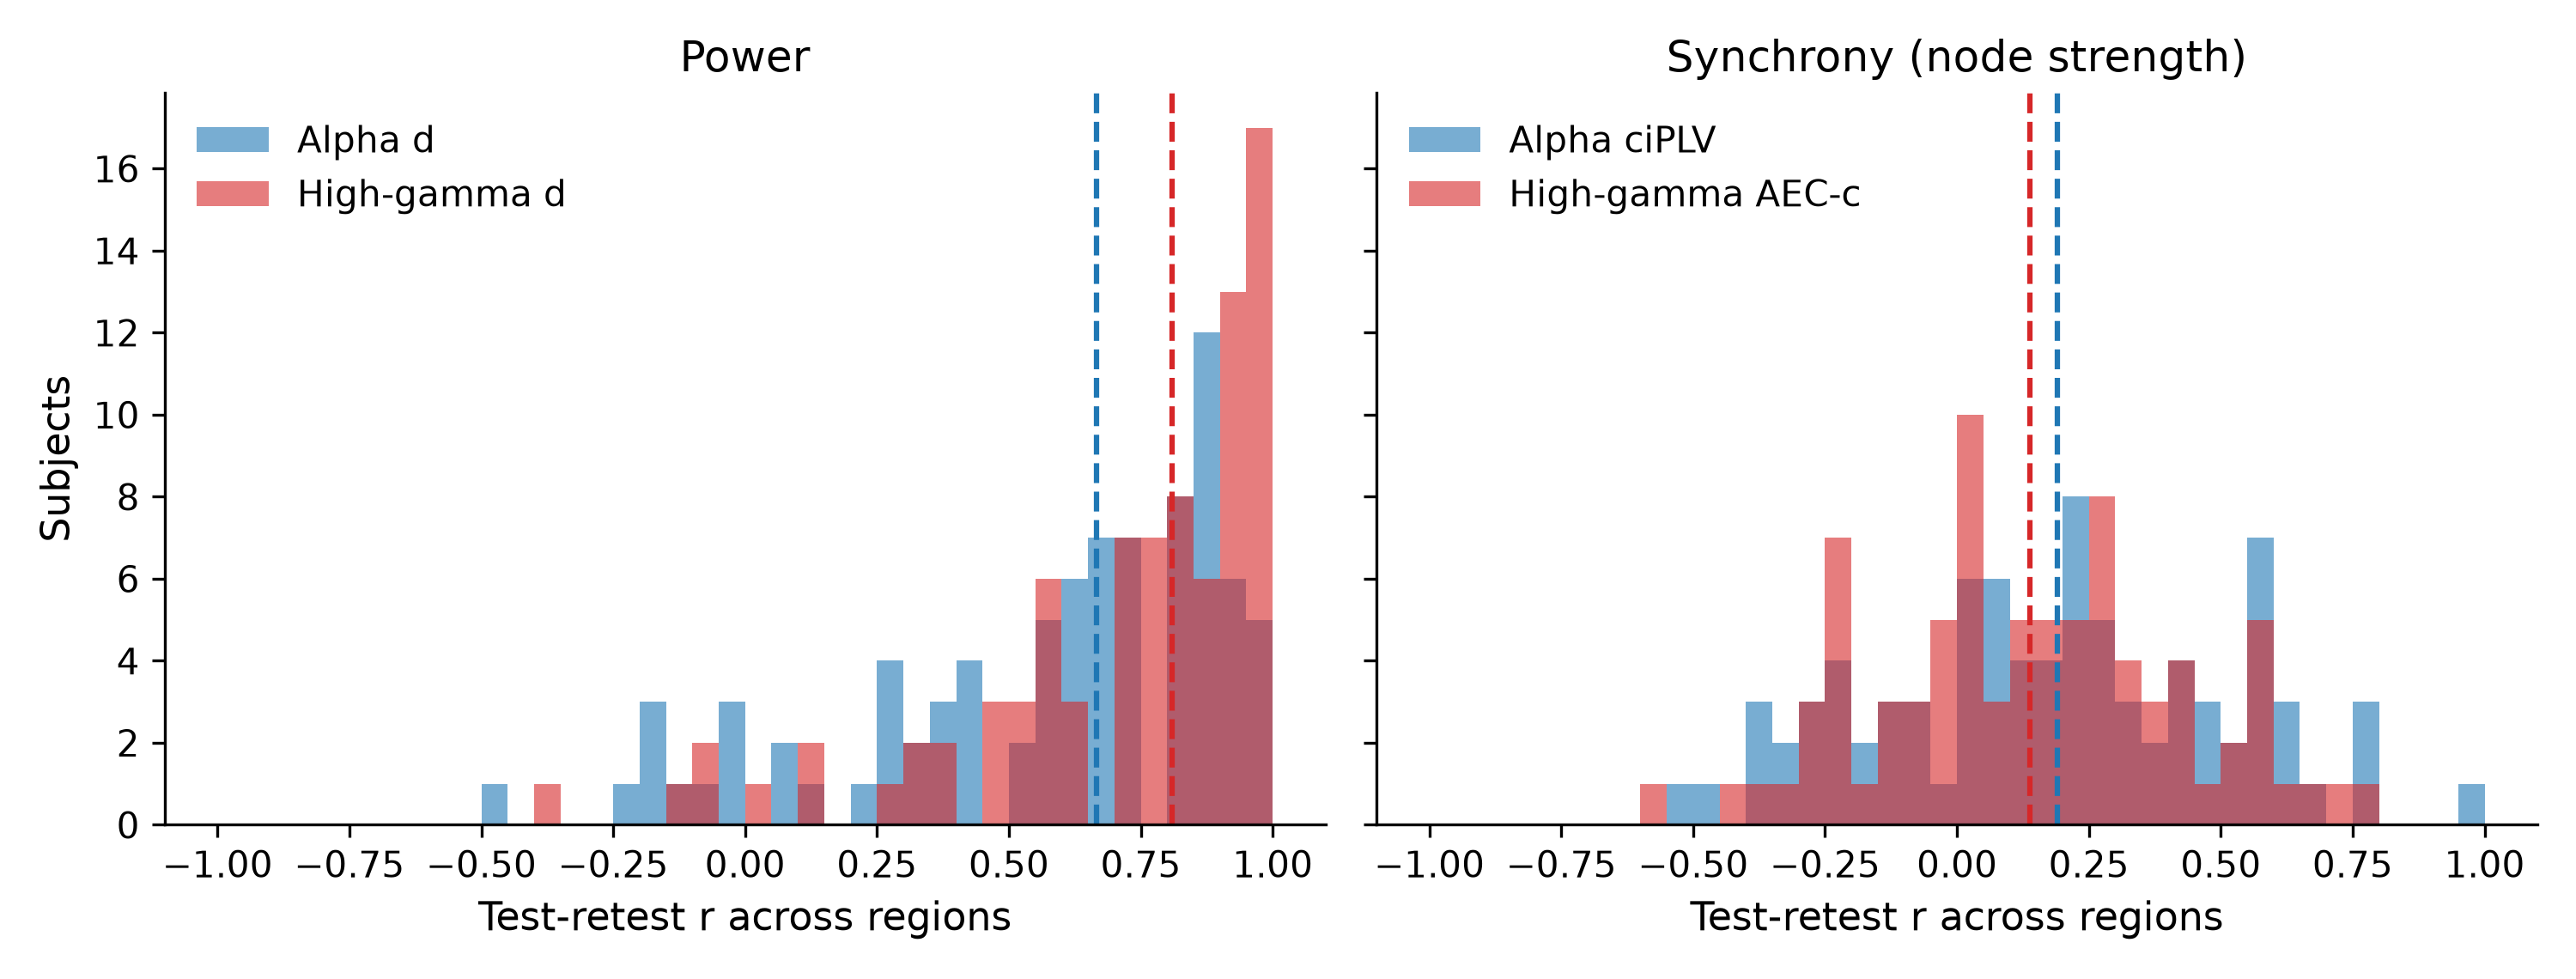
\includegraphics[keepaspectratio,alt={Reliability}]{img/fig8_reliability.png}}
\caption{Reliability}
\end{figure}

\begin{itemize}
\tightlist
\item
  87 subjects with $\geq$ 2 sessions per half. Power maps repeat: median r
  0.63 (alpha), 0.79 (high gamma). Synchrony maps much less: 0.16 (alpha
  ciPLV), 0.13 (high-gamma AEC-c). \textbf{(verify: CSV from 2026-10-14,
  script changed since)}
\end{itemize}

\subsection{Supplementary}\label{supplementary}

\begin{figure}
\centering
\pandocbounded{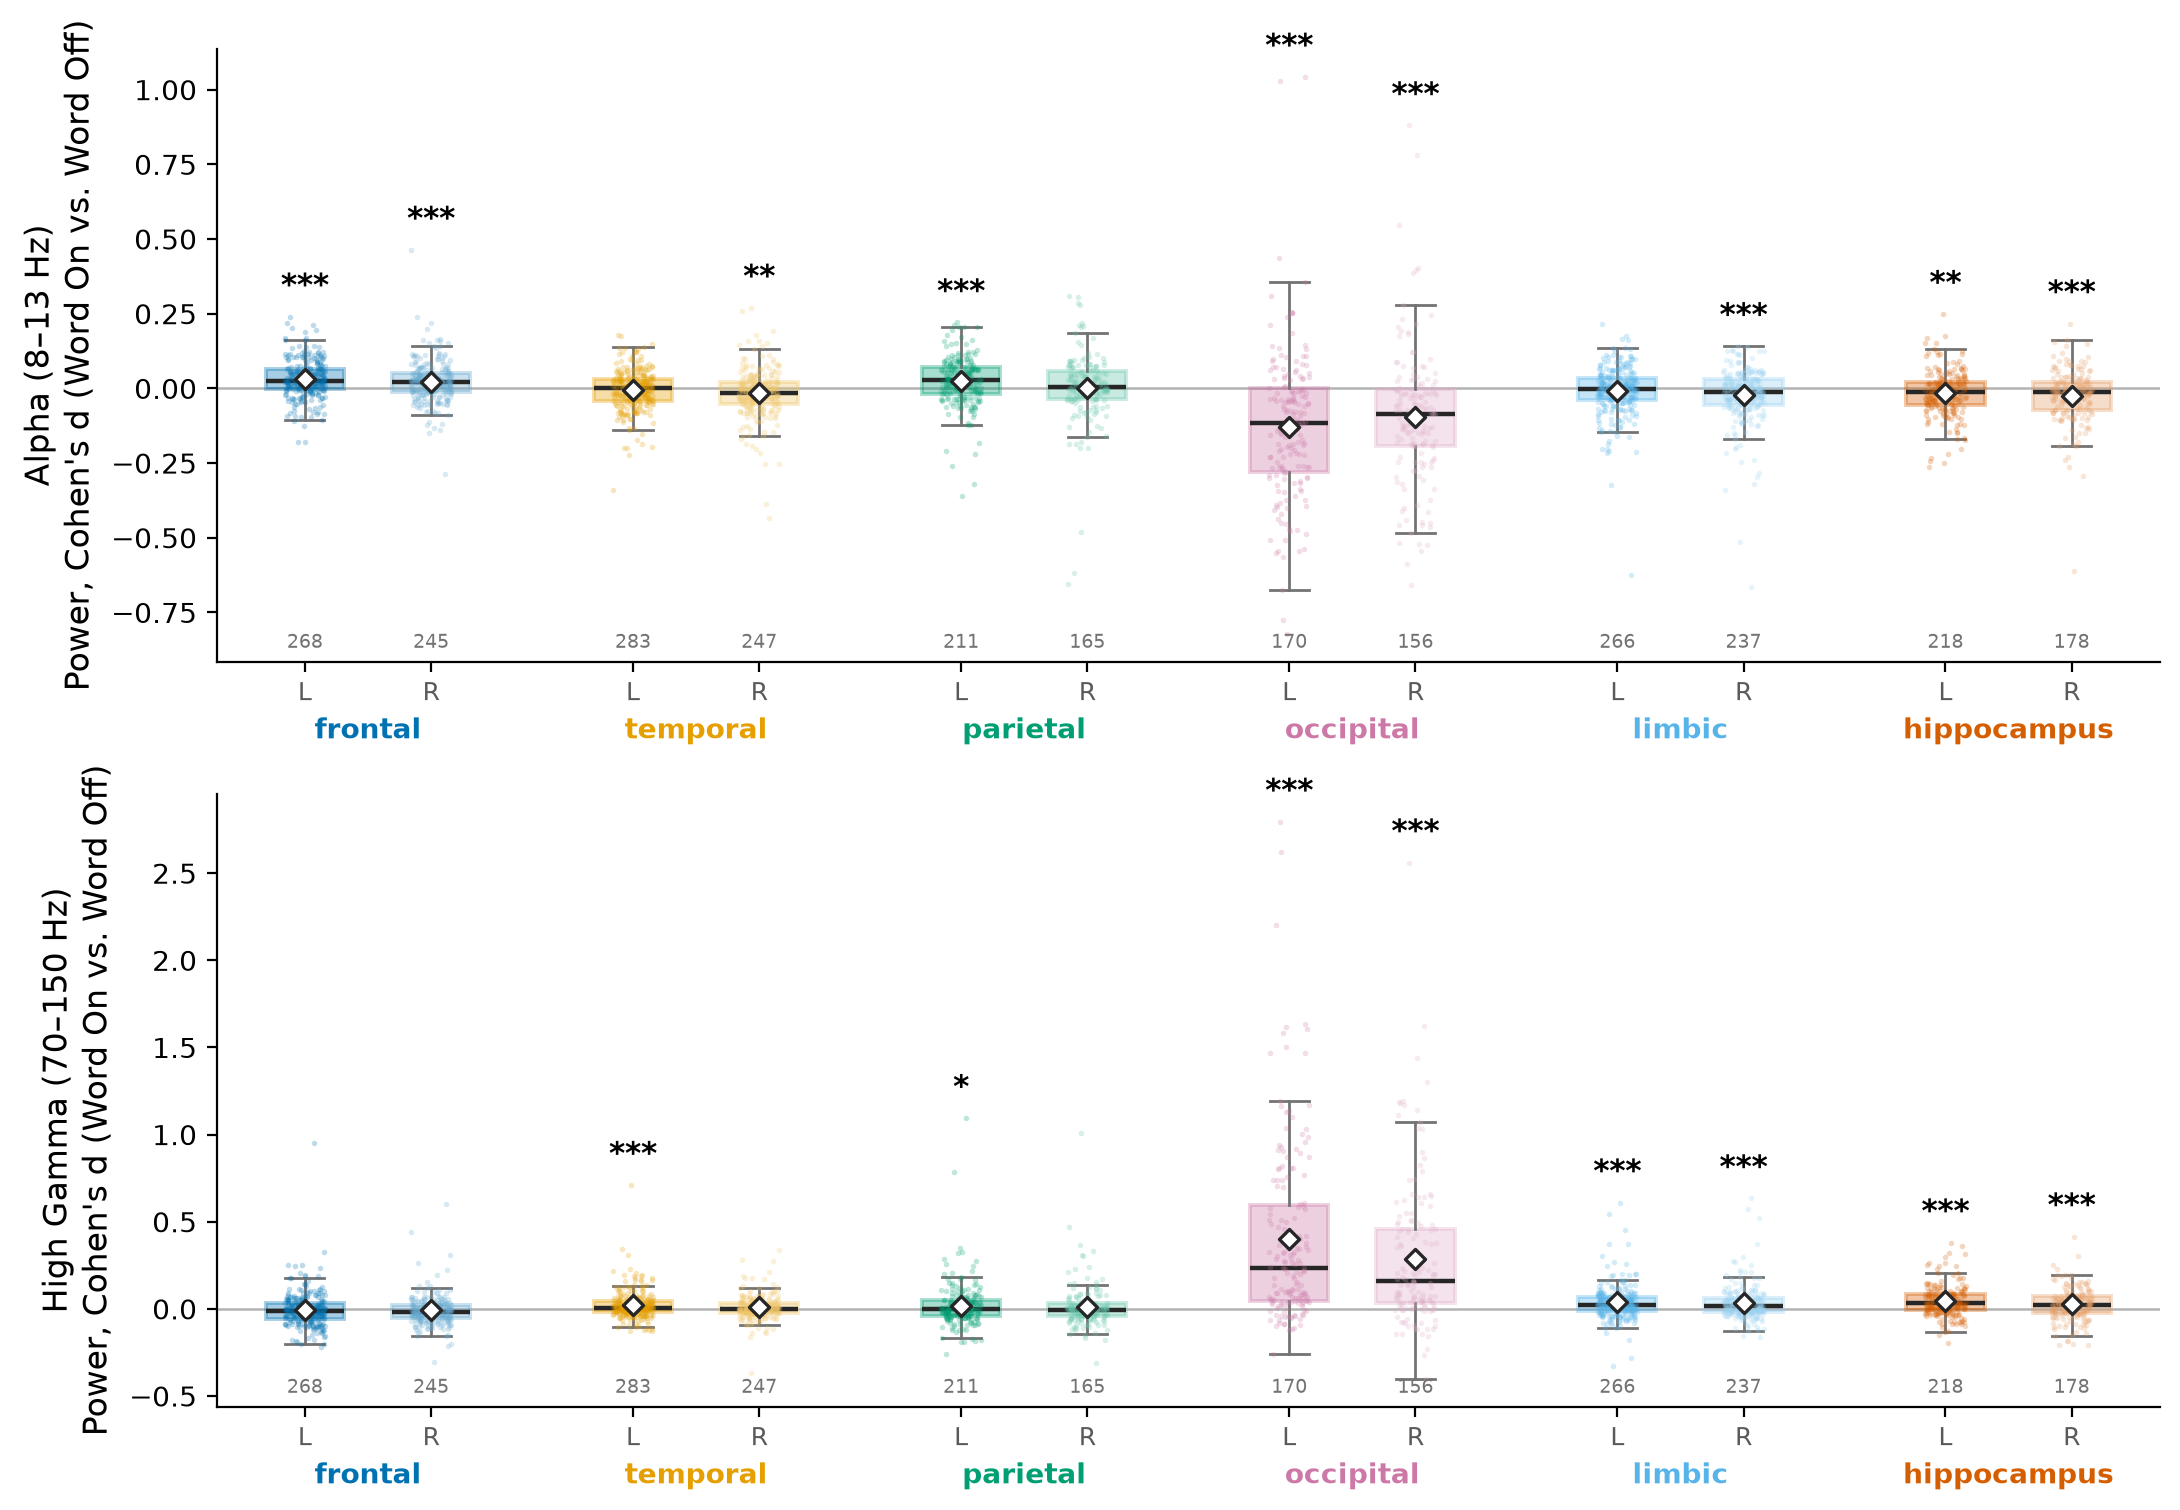
\includegraphics[keepaspectratio,alt={Power, subject
distributions}]{img/figS1_power_subjects.png}}
\caption{Power, subject distributions}
\end{figure}

\begin{figure}
\centering
\pandocbounded{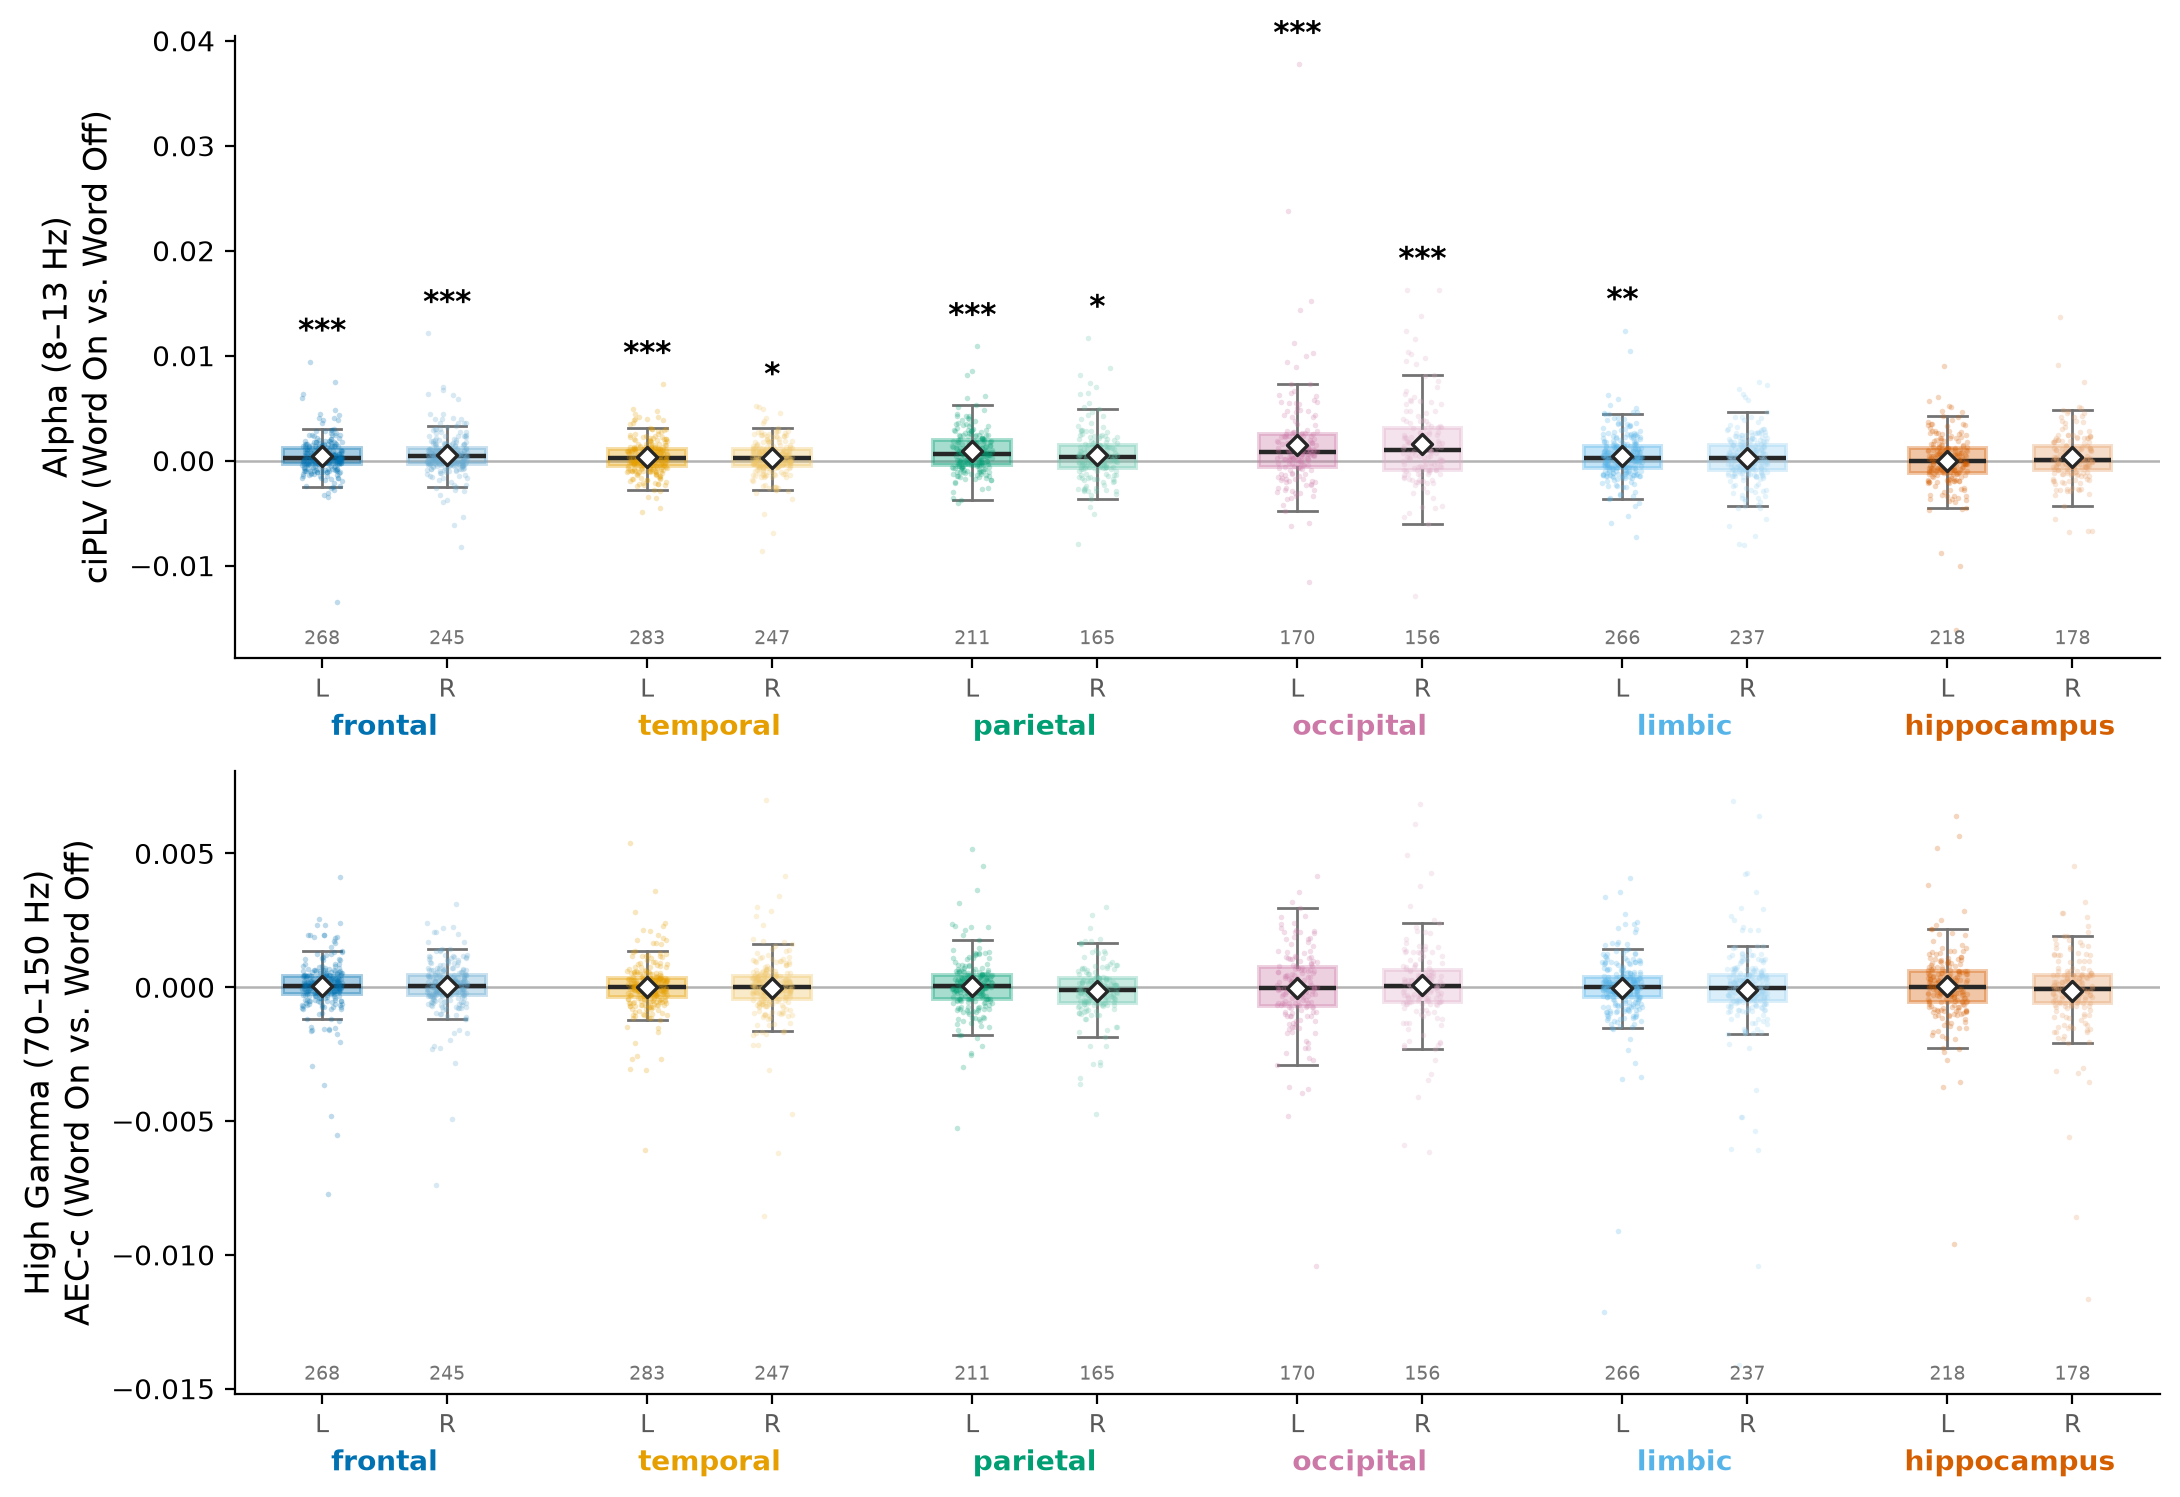
\includegraphics[keepaspectratio,alt={Synchrony, subject
distributions}]{img/figS2_synchrony_subjects.png}}
\caption{Synchrony, subject distributions}
\end{figure}

\subsection{Limitations / discussion}\label{limitations-discussion}

\begin{itemize}
\tightlist
\item
  Word-off baseline starts \textasciitilde80-410 ms after the previous
  word's offset: possible offset response / anticipation in the
  baseline; the blank-length split (Results 4) cannot separate the two.
\item
  No ERP subtraction: evoked activity contributes to power and
  synchrony, especially occipital.
\item
  Neighbour-transferred labels (\textasciitilde11\% / 21\% disagreement
  in LOSO).
\item
  High-gamma phase metrics avoided (broadband HFA has no meaningful
  phase); AEC-c null is consistent with high gamma being local and
  asynchronous (Solomon et al.~2017, 2019).
\item
  Multiple comparisons corrected within figures, not across.
\end{itemize}

\subsubsection{Stimulus-locked activity in
connectivity}\label{stimulus-locked-activity-in-connectivity}

\begin{itemize}
\tightlist
\item
  Subtracting the average ERP leaves a residual because amplitude and
  latency vary across trials: Truccolo et al.~2002; Wang, Chen \& Ding
  2008; Knuth et al.~2006.
\item
  Evoked and induced activity can't be cleanly separated: David et
  al.~2006; Shah et al.~2004. This supports the PI's position.
\item
  Is alpha phase reset? For: Makeig et al.~2002; Hanslmayr et al.~2007.
  Against: Mazaheri \& Jensen 2006. Hard to tell apart: Yeung et
  al.~2004; Sauseng et al.~2007.
\item
  Task-evoked activity inflates connectivity: Cole et al.~2019; van
  Diepen \& Mazaheri 2018; Kramer et al.~2008 (sharp transients).
\item
  Alternatives to subtraction:

  \begin{itemize}
  \tightlist
  \item
    Matched condition contrast with a label-shuffle null: Solomon et
    al.~2017; Maris et al.~2007.
  \item
    Trial-shuffled (shift-predictor) surrogates: Perkel et al.~1967;
    Aertsen et al.~1989; Brody 1999.
  \item
    Connectivity aligned to internal HFA peaks: Dede et al.~2025.
  \item
    Phase consistency on the same data: Colyer \& Kahana 2025.
  \end{itemize}
\end{itemize}

\end{document}
